% !TeX encoding = UTF-8
% !TeX spellcheck = es_ES
\documentclass[12pt]{article}
\usepackage{fullpage}
\usepackage[utf8]{inputenc}
\usepackage{pict2e}
\usepackage{amsmath}
\usepackage{enumitem}
\usepackage{eurosym}
\usepackage{mathtools}
\usepackage{amssymb, amsfonts, latexsym, cancel}
\setlength{\parskip}{0.3cm}
\usepackage{graphicx}
\usepackage{fontenc}
\usepackage{setspace}
\usepackage{adjustbox}
\setstretch{1.35}
\usepackage{bold-extra}
\usepackage{subcaption}
\graphicspath{ {images/} }
\usepackage{tcolorbox}
\usepackage{xcolor, colortbl}
\usepackage{wrapfig}
\usepackage{empheq}
\usepackage{array}
\usepackage{parskip}
\usepackage{arydshln}
\renewcommand*\contentsname{\color{black}Índice} 
\usepackage{array, multirow, multicol}
\definecolor{lightblue}{HTML}{007AFF}
\usepackage{color}
\usepackage{etoolbox}
\usepackage{listings}
\usepackage{mdframed}
\setlength{\parindent}{0pt}
\usepackage{underscore}
\usepackage{hyperref}
\usepackage{tikz}
\usetikzlibrary{shapes, positioning, patterns}
\usepackage{tikz-qtree}
\usepackage{biblatex}
\usepackage{pdfpages}
\usepackage{pgfplots}
\usepackage{pgfkeys}
\usepackage{mathrsfs}
\addbibresource{biblatex-examples.bib}
\usepackage[a4paper, left=1cm, right=1cm, top=1cm,
bottom=1.5cm]{geometry}
\everymath{\displaystyle}
\usetikzlibrary{decorations.pathreplacing}
\usepackage{titlesec}
\setlength{\fboxrule}{1.5pt}
\renewcommand{\arraystretch}{1.2}
\title{Cálculo I}
\author{Francisco Javier Mercader Martínez}
\date{}

% Configura el formato de las secciones utilizando titlesec
\titleformat{\section}
{\color{red}\normalfont\LARGE\bfseries}
{Tema \thesection:}
{10 pt}
{}

% Ajusta el formato de las entradas de la tabla de contenidos
\addtocontents{toc}{\protect\setcounter{tocdepth}{4}}
\addtocontents{toc}{\color{black}}

\titleformat{\subsection}
{\normalfont\Large\bfseries\color{red}}{\thesubsection)}{1em}{\color{lightblue}}

\titleformat{\subsubsection}
{\normalfont\large\bfseries\color{red}}{\thesubsubsection)}{1em}{\color{lightblue}}

\newcommand{\bboxed}[1]{\fcolorbox{lightblue}{lightblue!10}{$#1$}}

\newcommand{\bu}[1]{\textcolor{lightblue}{\underline{#1}}}
\newcommand{\lb}[1]{\textcolor{lightblue}{#1}}
\newcommand{\db}[1]{\textcolor{blue}{#1}}

\newcommand{\dx}{\:\mathrm{d}x}
\newcommand{\dt}{\:\mathrm{d}t}
\newcommand{\dy}{\:\mathrm{d}y}
\newcommand{\dz}{\:\mathrm{d}z}
\newcommand{\dth}{\:\mathrm{d}\theta}
\newcommand{\dr}{\:\mathrm{d}\rho}
\newcommand{\du}{\:\mathrm{d}u}
\newcommand{\dv}{\:\mathrm{d}v}
\newcommand{\tozero}[1]{\cancelto{0}{#1}}
\newcommand{\lbb}[2]{\textcolor{lightblue}{\underbracket[1pt]{\textcolor{black}{#1}}_{#2}}}
\newcommand{\dbb}[2]{\textcolor{blue}{\underbracket[1pt]{\textcolor{black}{#1}}_{#2}}}
\DeclareMathOperator{\N}{\mathbb{N}}
\DeclareMathOperator{\Z}{\mathbb{Z}}
\DeclareMathOperator{\R}{\mathbb{R}}
\DeclareMathOperator{\Q}{\mathbb{Q}}
\DeclareMathOperator{\K}{\mathbb{K}}

\renewcommand{\CancelColor}{\color{lightblue}}
\begin{document}
\maketitle
{\setstretch{1.45} \tableofcontents}
\newpage
\section{Los números naturales}

\subsection{Los números naturales}

Hemos trabajado con ellos desde que apenas tenemos memoria. Hemos aprendido a contar \[ 1,2,3,4,\hdots,n,\hdots\]
Con un orden, \[ 1<2<3<\cdots<n-1<n<n+1 \]
Denotaremos dicho conjunto como $\mathbb{N}$
\begin{itemize}[label=\color{red}\textbullet, leftmargin=*]
	\item \color{lightblue} Propiedades
\end{itemize}
\begin{enumerate}[label=\arabic*)]
	\item Es infinito. Su cardinal es el infinito "más pequeño". Un conjunto para el que existe una biyección con el de los números naturales recibe el nombre de \textit{conjunto numerable}.
	\item Todo subconjunto de $\mathbb{N}$ tiene un elemento mínimo. En esta propiedad se basa el "Principio de Inducción".
\end{enumerate}
Vamos a empezar realizando alguna pequeña demostración utilizando el principio de inducción.
\subsubsection{El Principio de Inducción}
\begin{itemize}[label=\color{red}\textbullet, leftmargin=*]
	\item \color{lightblue} Proposición
\end{itemize}
Supongamos que de una determinada propiedad $P(n)$, en la cual interviene un número natural genérico $n$, si:
\begin{enumerate}[label=\arabic*)]
	\item La propiedad es cierta para $n=1$.
	\item Se supone que la propiedad es cierta para un número $n$ (hipótesis de inducción) se deduce que la propiedad es cierta para $n+1$.
\end{enumerate}
Entonces la propiedad $P(n)$ es cierta para todo número natural $n$.

\begin{itemize}[label=\color{red}\textbullet, leftmargin=*]
	\item \color{lightblue} Ejercicio
\end{itemize}
Establecer la igualdad \[ 1+2+3+\cdots+n=\dfrac{n(n+1)}{2} \]
Para $n\ge 1$ (también lo podemos indicar de la forma $n\in\mathbb{N}$).

Establecer la igualdad \[ a+a^2+\cdots+a^n=\dfrac{a-a^{n+1}}{1-a},~a\neq1 \] para $n\ge1$.

Como sabemos, \[ \mathbb{N}\subset\mathbb{Z}\subset\mathbb{Q}\subset\mathbb{R} \]
\subsection{Los números reales}
Los números reales aparecen de forma natural. ¿Cuál es la solución de la ecuación $x^2=2$?

Observa que la solución no puede ser un número racional, ya que si $x=\dfrac{m}{n}$ siendo $m,n\in\mathbb{N}$, en cuyo caso \[ \dfrac{m^2}{n^2}=2, \]\[ m^2=2n^2, \]
Lo cual nos indica que la descomposición factorial del término de la izquierda habrá una potencia par de 2, mientras que en el término de la derecha de la igualdad el número será impar, de donde se sigue que la ecuación no tiene soluciones racionales.

Otro problema, en cuanto a la idea de que algo es necesario si nos quedamos únicamente con los racionales viene dada por el siguiente ejemplo.

Supongamos que $A$ es un conjunto que viene dado por

$A:=\{p\in\mathbb{Q}:p^2<2\}$ y $B$ es el conjunto dado por:

$B=\{p\in\mathbb{Q}:p^2>2\}$. En estos casos es posible demostrar que $A$ no tiene máximo (y $B$ no tiene mínimo), es decir, para cada $p\in A$, existe $q\in A$ tal $p<q$. Veremos las definiciones formales de máximo y mínimo de un conjunto más adelante.

Para demostrar esta afirmación para cada número racional $p>0$ consideramos el número racional $q$ dado de la forma \[ q=p-\dfrac{p^2-2}{p+2}=\dfrac{p^2+2p-p^2+2}{p+2}=\dfrac{2(p+1)}{p+2}. \]
Ahora, \[ q^2-2=\dfrac{4(p+1)^2}{(p+2)^2}-2=\dfrac{4(p^2+1+2p)-2(p^2+4+4p)}{(p+2)^2}=\dfrac{2(p^2-2)}{(p+2)^2}.\]
Si $p\in A$, entonces el numerador de la expresión anterior es negativo, es decir, $p^2-2<0$, y de ahí $q\in A$, pero por otra parte $q>p$ por la propia definición de $q$. Luego para cada $p\in A$ es posible encontrar $q\in A$ tal que $q>p$. La misma demostración se puede aplicar para el caso de $B$.

\subsubsection{Construcción de los números reales}
La construcción de los números reales puede abordarse como una ampliación partiendo de los números naturales, los números racionales y los números negativos (mediante sucesiones de números racionales), no obstante, nosotros utilizaremos la definición axiomática.

\subsection{Definición axiomática de los número reales}
Antes de dar la definición axiomática de los números reales necesitamos precisar algunos conceptos que necesitaremos.
\begin{itemize}[label=\color{red}\textbullet, leftmargin=*]
	\item \color{lightblue} Definición
\end{itemize}
Un cuerpo es una terna $(K,+,\cdot)$ donde $K$ es un conjunto no vacío y $+,\cdot$ son leyes de composición internas en $K$ tales que:
\begin{enumerate}[label=\arabic*)]
	\item $(K,+)$ es un grupo abeliano. Denotaremos por 0 el elemento neutro de $K$ y si $a\in K$ denotaremos por $-a$ al simétrico de $a$.
	\begin{enumerate}[label=\alph*)]
		\item $\cdot$ es asociativa.
		\item  $\cdot$ es conmutativa.
		\item Existe $1\in K\{0\}$ tal que $1\cdot a=a~~\forall a\in K\{0\}$.
		\item $\forall a\in K\{0\}$ existe $a^{-1}\in K\{0\}$ tal que $a^{-1}\cdot a=1$. A $a^{-1}$ le llamaremos el inverso de $a$.
		\item $a\cdot(b+c)=a\cdot b+a\cdot c~~\forall a,b,c\in K$.
	\end{enumerate}
\end{enumerate}
\begin{itemize}[label=\color{red}\textbullet, leftmargin=*]
	\item \color{lightblue} Definición
\end{itemize}
Dado $A$ un conjunto, una relación binaria $\le$ en $A$ se dice que es una relación binaria de orden si verifica:
\begin{enumerate}[label=\arabic*)]
	\item $a\le a~~\forall a\in A$. (Propiedad Reflexiva).
	\item Si $a,b\in A$ tal que $a\le b\wedge b\le a\rightarrow a=b$. (Propiedad Antisimétrica).
	\item Si $a,b,c\in A$ tal que $a\le b\wedge b\le c\rightarrow a\le c$. (Propiedad transitiva).
\end{enumerate}
Un conjunto ordenado es un par $(A,\le)$ donde $A$ es un conjunto y $\le$ es una relación binaria de orden definida en $A$.

\textbf{¿Qué cuerpos conoces?}

Fíjate en el conjunto $A=\{0,1\}$ con las operaciones:
\begin{center}
	\begin{tabular}{|c|c|c|}
		\hline
		+ & 0 & 1 \\
		\hline
		0 & 0 & 1 \\
		\hline
		1 & 1 & 0 \\
		\hline
	\end{tabular}\hspace{3cm}
	\begin{tabular}{|c|c|c|}
		\hline
		* & 0 & 1 \\
		\hline
		0 & 0 & 0 \\
		\hline
		1 & 0 & 1 \\
		\hline
	\end{tabular}
\end{center}
\textbf{¿Es $\mathbb{N}$ un cuerpo? ¿Es $\mathbb{Q}$ un cuerpo?}

Otro concepto a tener en cuenta es el \textbf{"orden"}. Recordaremos algunos conceptos. 

Veamos:
\begin{itemize}[label=\color{red}\textbullet, leftmargin=*]
	\item \color{lightblue} Definición
\end{itemize}
Sea $(A,\le)$ un conjunto ordenado, $B\subseteq A$ y $a\in A$.
\begin{enumerate}[label=\arabic*)]
	\item Diremos que $a$ es cota superior de $B$ si $b\le a$ para cada $b\in B$.
	\item Diremos que $a$ es cota inferior de $B$ si $a\le b$ para cada $b\in B$.
	\item Diremos que $a$ es el supremo de $B$ si:
	\begin{enumerate}[label=\arabic*)]
		\item $a$ es cota superior de $B$.
		\item Si $a'$ es otra cota superior de $B$ entonces $a\le a'$.
	\end{enumerate}
	\item Diremos que $a$ es el ínfimo de $B$ si:
	\begin{enumerate}[label=\arabic*)]
		\item $a$ es cota inferior de $B$.
		\item Si $a'$ es otra cota inferior de $B$ entonces $a'\le a$.
	\end{enumerate}
\end{enumerate}
Sea $A$ un conjunto ordenado, $B\subseteq A$ y $b\in B$.
\begin{enumerate}[label=\arabic*)]
	\item Diremos que $b$ es un elemento maximal (o máximo) de $B$ si no existe $b'\in B$ con $b\le b'$ y $b\neq b'$.
	\item Diremos que $b$ es un elemento minimal (o mínimo) de $B$ si no existe $b'\in B$ con $b'\le b$ y $b\neq b'$.
\end{enumerate}
\begin{itemize}[label=\color{red}\textbullet, leftmargin=*]
	\item \color{lightblue} Definición
\end{itemize} 
Llamaremos \textcolor{lightblue}{conjunto de los números reales} a un conjunto, que representaremos por $\mathbb{R}$, que verifica los siguientes axiomas:
\begin{enumerate}[label=\arabic*)]
	\item El conjunto $\mathbb{R}$ tiene estructura de cuerpo.
	\item En $\mathbb{R}$ hay definida una relación de orden, (es decir, una relación que verifica las propiedades reflexivas, antisimétrica y transitiva) que es total (siempre se verifica $x\le y$ o bien $y\le x$) para cualesquiera $x,y\in\mathbb{R}$ y compatible con la estructura de cuerpo (si $x\le y$ entonces $x+z\le y+z$, y si $z\ge0$, entonces $xz\le yz$).
	\item Existencia de supremo en $\mathbb{R}$. Todo conjunto no vacío de $\mathbb{R}$ acotado superiormente tiene extremo superior (supremo) en $\mathbb{R}$.
\end{enumerate}
El siguiente paso sería asegurarnos de la existencia del conjunto de los números reales, sin embargo, no nos ocuparemos aquí de ese paso. Remitimos al lector a algunas referencias en donde algunas construcciones clásicas como el método de las cortaduras en $\mathbb{Q}$ de Dedekind (1831-1916) y la construcción de Cantor (1845-1918) utilizando sucesiones de Cauchy de números racionales son algunas posibilidades. 

Ver por ejemplo \textit{Constructions of the real numbers}. 

Los elementos de $\mathbb{R}\backslash\mathbb{Q}$ se llaman \textit{irracionales}, y los denotaremos por $\mathbb{I}$. Más adelante hablaremos de ellos y de su cardinal. Habitualmente los números reales se representan por medio de puntos de una recta. Se elige un punto para representar el 0 y otra para representar la unidad 1. Esta elección determina la escala. El orden de los números viene dado por su representación en la recta.
\begin{itemize}[label=\color{red}\textbullet, leftmargin=*]
	\item \color{lightblue} Proposición (Propiedad arquimediana de los números reales)
\end{itemize}
Para cada par de elementos $x,y\in\mathbb{R}$, tal que $x>0$, existe $n\in\mathbb{Z}$ tal que $y<nx$.
\begin{itemize}[label=\color{red}\textbullet, leftmargin=*]
	\item \color{lightblue} Demostración
\end{itemize}
Sea el conjunto $A=\{mx:m\in\mathbb{Z}\}$. Supongamos que la afirmación no fuera cierta, es decir, para todo $n\in\mathbb{Z}$ y $y>mx$, luego el conjunto $A$ está acotado superiormente. Por el axioma del supremos existe $\alpha\in\mathrm{R}$ tal que $\alpha=\mathrm{sup}(A)$. Puesto que $x>0$, tenemos que $\alpha-x<\alpha$, luego existe $s\in\mathbb{Z}$ tal que $\alpha-x<sx$ y así: \[ a<sx+x=(s+1)x, \]lo cual es absurdo puesto que $\alpha$ es el supremo de $A$. De aquí deducimos que la propiedad es cierta. 

Apoyándonos en la propiedad arquimediana podemos afirmar que para cada número real $y\in\mathbb{R}$ y $x\in\mathbb{R}$ y $x>0$, existen $m,n\in\mathbb{Z}$ tales que \[ mx<y<nx \]
Es decir, \[ mx<(m+1)x<\cdots<px<\cdots<(n-1)x<nx \]
Luego existirá un entero $p\in\mathbb{Z}$ tal que \[ (p-1)x\le y<px \]
Tomando $x=1$, podemos entonces asegurar la existencia de un entero $p$ tal que \[ p-1\le y<p \]
\begin{itemize}[label=\color{red}\textbullet, leftmargin=*]
	\item \color{lightblue} Definición
\end{itemize}
Al número $p-1\in\mathbb{Z}$ se le llama parte entera de $y$ y se le denota $E(y)$ o $[y]$.
\subsection{Valor absoluto}
\begin{itemize}[label=\color{red}\textbullet, leftmargin=*]
	\item \color{lightblue}Definición
\end{itemize}
Se llama valor absoluto de $x\in\mathbb{R}$ al número real denotado por $|x|$ dado por \[ |x|=\max\{x,-x\} .\]
Es decir, \[ |x|=\left\lbrace\begin{array}{cl}
	x & \text{si }x\ge0\\
	-x & \text{si }x<0
\end{array}\right. .\]
\subsubsection{Propiedades del valor absoluto}
\begin{itemize}[label=\color{red}\textbullet, leftmargin=*]
	\item \color{lightblue}Proposición
\end{itemize}
\begin{enumerate}[label=\arabic*)]
	\item $|-x|=|x|$.
	\item Para cada $\epsilon>0,~|x|<\epsilon$ es equivalente a $-\epsilon<x<\epsilon$.
	\item $|x|=0$ si y sólo si $x=0$.
	\item $|x+y|\le |x|+|y|$.
	\item $|x-y|\ge|x|-|y|$.
	\item $|x\cdot y|=|x|\cdot|y|$.
	\item $|x^{-1}|=|x|^{-1}$ para cada $x\neq0$.
	\item $\left||x|-|y|\right|\le|x-y|$.
\end{enumerate}
Probaremos únicamente las propiedades \textcolor{lightblue}{(4)} y \textcolor{lightblue}{(5)}:
\begin{enumerate}[label=\arabic*)]
	\item $|x+y|=\max\{x+y,~x-y\}$. Por otro lado $-|x|\le x\le |x|$ y $-|y|\le y\le |y|$, luego $-\left(|x|+|y|\right)\le x+y\le |x|+|y|$ y por la propiedad \textcolor{lightblue}{(2)} tenemos que $|x+y|<|x|+|y|$.
	\item $x=x-y+y$, de donde \[ |x|=\left|(x-y)+y\right|\le|x-y|+|y|, \]de donde, $|x|-|y|\le|x-y|$.
\end{enumerate}
\subsection{Densidad}
\begin{itemize}[label=\color{red}\textbullet, leftmargin=*]
	\item \color{lightblue} Proposición (Densidad de $\mathbb{Q}$ y $\mathbb{I}$)
\end{itemize}
\begin{enumerate}[label=\arabic*)]
	\item Sean $x,y\in\mathbb{R}$ tales que $x<y$. Entonces existe $r\in\mathbb{Q}$ tal que $x<r<y$.
	\item Dados $r,s\in\mathbb{Q}$ tales que $r<s$. Entonces existe $\xi\in\mathbb{I}$ tal que $r<\xi<s$.
\end{enumerate}
Por la propiedad arquimediana, dados $y-x>0$ y $1$, existe $n\in\mathbb{N}$ tal que \[ 1<n(y-x) .\]
Sea $p=E(nx)\in\mathbb{Z}$. Entonces se verifica que $p\le nx<(p+1)$, luego \[ nx<p+1\le nx+1<ny ,\] de donde \[ nx<p+1<ny \] o de forma equivalente \[ x<\dfrac{p+1}{n} <y.\]
Es decir $r=\dfrac{p+1}{n}\in\mathbb{Q}$ verifica la condición buscada. Aplicando a la misma propiedad a $x<r$ podemos afirmar la existencia de $s\in\mathbb{Q}$ tal que $x<s<r$ lo cual muestra  que existen infinitos números racionales cumpliendo la condición del enunciado.

Por otra parte, es posible demostrar que entre dos números racionales $r<s$ existen infinitos irracionales. Sabemos que el número $b\in\mathbb{R}$ tal que $b^2=2$ es irracional y que $b<2$. Entonces, el número $a=\dfrac{b(s-r)}{2}$ es irracional y tenemos que $a<s-r$. Ahora el número $\xi=r+a$ es irracional y $r<\xi<s$.
\subsection{Representación decimal de los números reales}
\begin{itemize}[label=\color{red}\textbullet, leftmargin=*]
	\item \color{lightblue} Definición
\end{itemize}
Se llama números algebraicos a aquellos que son raíces de alguna ecuación polinómica con coeficientes enteros. Los números que no son algebraicos se llaman trascendentes.

Un número real de la forma \[ r=a_0+\dfrac{a_1}{10}+\dfrac{a_2}{100}+\cdots+\dfrac{a_n}{10^n} ,\] donde $a_0$ es un entero no negativo y $a_1,a_2,\hdots,a_n$ son enteros que satisfacen $0\le a_i\le 9$ se escribe de la forma \[ r=a_0,a_1,a_2,\hdots,a_n. \]
En este caso tendríamos una representación decimal finita y el número $r$ es necesariamente racional.

Sin embargo, no todos los números racionales tienen una representación decimal finita. Así, si $\dfrac{1}{3}$ tuviera representación decimal finita tendríamos que $\dfrac{1}{3}=\dfrac{a}{10^n}$ para cierto $a$ y cierto $n$, es decir, $10^n=3a$ lo cual no es posible, puesto que 3 no es divisor de ninguna potencia de 10.

Sin embargo, podemos aproximar cualquier número real $x>0$ por una aproximación decimal con un error tan pequeño como se desee por medio de una suma como la expresada anteriormente basándonos en el hecho de ir dividiendo el intervalo en 10 partes iguales en cada paso de forma que 

\[\begin{array}{rcl}
	a_0&\le x<&a_0+1 \\
	a_0+\dfrac{a_1}{10}&\le x<&a_0+\dfrac{a_1+1}{10}\\
	a_0+\dfrac{a_1}{10}+\dfrac{a_2}{100}+\dfrac{a_2}{100}&\le x<&a_0+\dfrac{a_1}{10}+\dfrac{a_2+1}{100}\\
	&\cdots&
\end{array}\]

Cada número irracional tiene una representación decimal infinita. Observar que es importar tener en cuenta en esta definición dónde situamos la posibilidad de igualdad, ya que utilizando esta situación la representación de $\dfrac{1}{8}$ sería \[ \begin{array}{c}
	0\le\frac{1}{8}<1,\\
	\frac{1}{10}\le \dfrac{1}{8}<\frac{2}{10}\\
	\frac{1}{10}+\frac{2}{100}\le\frac{1}{8}<\frac{1}{10}+\frac{3}{100}\\
	\frac{1}{10}+\frac{2}{100}+\frac{5}{1000}\le\frac{1}{10}+\frac{2}{100}+\frac{6}{1000}
\end{array} \] y la representación de $\frac{1}{8}$ sería $0.125$, sin embargo si colocamos el signo menor estricto en lugar de menor o igual e incluimos la posibilidad de que sea mayor o igual por exceso tendríamos que la representación de $\frac{1}{8}$ sería $ 0.1249999\hdots$  Hemos obtenido de esta forma dos representaciones distintas para el mismo número.

\subsubsection{La representación de los números reales en el ordenador (Python)}
La representación de los números reales en el ordenador. La cantidad de números con los que el ordenador puede trabajar es finita. Esta afirmación debemos tenerla en cuenta cada vez que pensamos en simulaciones pero no sólo eso, también es importante tener en cuenta cómo trabaja y/o almacena en un ordenador un número.
 En Python la clase "float" (64 bits):
 \begin{itemize}
 	\item 1 bit para el signo del número (positivo o negativo).
 	\item  11 bits para el exponente (el rango es $[-1022, 1023]$).
 	\item 53 bits para dígitos significativos.
 \end{itemize}
 \subsection{Cardinal de un conjunto}
 Se llama \textit{cardinal} de un conjunto $A$ al número de elementos de dicho conjunto y se denota $|A|$.
 
 El conjunto vacío, es decir, de cardinal cero se denota por $\varnothing$.
 
 \begin{itemize}[label=\color{red}\textbullet, leftmargin=*]
 	\item \color{lightblue} Definición
 \end{itemize}
 Diremos que un conjunto $B$ es un subconjunto o parte de un subconjunto $A$ o que $B$ está contenido en $A$ si, todos los elementos de $B$ son a su vez elementos de $A$. Es decir, \[ B\subseteq A\longleftrightarrow x\in B\rightarrow x\in A \]
 Un conjunto $A$ de elementos cualesquiera se dice numerable cuando es finito o cuando siendo finito existe una biyección de $A$ sobre el conjunto de los números naturales $\mathbb{N}$.
 \begin{itemize}[label=\color{red}\textbullet, leftmargin=*]
 	\item \color{lightblue}Proposición
 \end{itemize}
 El conjunto de los números racionales, $\mathbb{Q}$, es numerable.
 
 \begin{itemize}[label=\color{red}\textbullet, leftmargin=*]
 	\item \color{lightblue}Demostración
 \end{itemize}
 Sea $Q_k$  el conjunto de todas las fracciones del denominador $k\in\mathbb{N}$. El subconjunto $Q_k^+$ de las que tienen numerador positivo es trivialmente numerable. De igual forma el conjunto $Q_k^-$ de las que tienen numerador negativo también es numerable y así $Q_k=Q_k^-\cup\{0\}\cup Q_k^+$ es numerable. Ahora el conjunto $\mathbb{Q}=\cup_{k\in\mathbb{N}}Q_k$ es numerable.
 
 El cardinal de los números reales recibe el nombre de potencia del uso continuo. Se dice que un conjunto tiene la potencia del conjunto si existe una biyección de dicho conjunto sobre el $\mathbb{R}$. Durante muchos años estuvo planteado (primer problema de Hilbert) el problema de averiguar si existe subconjuntos de $\mathbb{R}$ que no sean numerables ni tengan la potencia del continuo, es decir $|\mathbb{R}|=\aleph_1$. Finalmente se ha demostrado que no se puede dar una respuesta ni afirmativa ni negativa a partir de los axiomas de definición del cuerpo de los números reales. El admitir este supuesto se convierte en una verdadera hipótesis, (hipótesis del continuo).
 \subsection{La idea del infinito}
 Se llama ampliación de $\mathbb{R}$ al conjunto $\overline{\mathbb{R}}=\mathbb{R}\cup\{-\infty,~\infty\}$ y se admite que $-\infty<x<+\infty$ para cada $x\in\mathbb{R}$.
 \begin{itemize}
 	\item $x+(+\infty)=x-(-\infty)=+\infty;~x+(-\infty)=x-(+\infty)=-\infty$.
 	\item Si $x>0,~x\cdot(+\infty)=(+\infty)\cdot x=+\infty$; si $x<0$, entonces $x\cdot(+\infty)=(+\infty)\cdot x=-\infty$.
 	\item Si $x>0,~x\cdot(+\infty)=(-\infty)\cdot x=-\infty$; si $x<0,~x\cdot(-\infty)=(-\infty)\cdot x=+\infty$.
 	\item $\frac{x}{+\infty}=\frac{x}{-\infty}=0$.
 	\item $(+\infty)+(+\infty)=(+\infty)-(-\infty)=(+\infty)\cdot(+\infty)=(-\infty)\cdot(-\infty)=+\infty$.
 	\item $(-\infty)+(-\infty)=(-\infty)-(-\infty)=(-\infty)\cdot(+\infty)=(+\infty)\cdot(-\infty)=-\infty$.
 \end{itemize}
\subsection{Funciones elementales}
\begin{itemize}[label=\color{red}\textbullet, leftmargin=*]
	\item \color{lightblue}Definición
\end{itemize} 
Sea $I\subset\mathbb{R}$. Se llama función real de variable real a toda aplicación $f:I\Rightarrow\mathbb{R}$ tal que $y=f(x)$. $x$ recibe el nombre de variable independiente y el nombre de variable dependiente. Al conjunto $I$ se llama conjunto inicial y al conjunto $\{f(x):x\in I\}$ se le llama conjunto imagen de $I$ mediante $f$. Al conjunto de valores en que la función se encuentra bien definida se le llama dominio de definición de $f$.

Seguimos algunas nociones conocidas:
\begin{itemize}[label=\color{red}\textbullet, leftmargin=*]
	\item \color{lightblue}Definición
\end{itemize}
Una función $f:I\Rightarrow\mathbb{R}$ se dice que es:
\begin{itemize}
	\item  Par si $f(x)=f(-x)$ para cada $x\in I$.
	\item Impar si $f(x)=-f(x)$ para cada $x\in I$.
	\item Creciente si para $x<y$ entonces $f(x)\le f(y)$.
	\item Estrictamente creciente si para $x<y$ entonces $f(x)<f(y)$.
	\item Decreciente si para $x<y$ entonces $f(x)\ge f(y)$.
	\item Estrictamente decreciente si para $x<y$ entonces $f(x)>f(y)$.
\end{itemize}
\subsubsection{Potencias de base real y exponente entero}
\fbox{$f(x)=x^n$}
\begin{itemize}[label=\color{red}\textbullet, leftmargin=*]
	\item \color{lightblue}Proposición (Propiedades)
\end{itemize}
\begin{itemize}
	\item  Si $n>0$ entonces $x^n=x\cdot x\cdot~\cdots~\cdot x$.
	\item Si $n=0,~x^0=1$.
	\item Si $n<0$ entonces $x^n=\dfrac{1}{x^{-n}}$.
	\item $(xy)^n=x^n\cdot y^n$.
	\item $x^n\cdot x^m=x^{n+m}$.
	\item $ \left(x^n\right)^m=x^{n\cdot m}$.
	\item Si $n>0$, entonces $x^n$ es monótona creciente en $(0,+\infty)$
	\item Si $n<0,~x^n$ es monótona decreciente en $(0,-\infty)$
\end{itemize}
\subsubsection{Función exponencial}
Sea $a>0$, se define la función exponencial $f(x)=a^x$.
\begin{itemize}[label=\color{red}\textbullet, leftmargin=*]
	\item \color{lightblue}Proposición (Propiedades)
\end{itemize}
\begin{itemize}
	\item Si $a=1$, la función es constantemente igual a 1.
	\item $a^{x+y}=a^x\cdot a^y,~a^0=1$.
	\item Si $x<y$ y $0<a<1$, entonces $a^y<a^x$.
	\item Si $a>1,~\lim_{x\to\infty}a^x=+\infty,~\lim_{x\to-\infty}a^x=0$.
	\item Si $0<a<1,~\lim_{x\to\infty}a^x=0,~\lim_{x\to-\infty}a^x=+\infty$.
\end{itemize}
\subsubsection{Función logaritmo}
Sea $a>0~f(x)=\log_a(x)$

De aquí,  $y=\log_a(x)$ sí, y sólo si, $a^y=x$.
\begin{itemize}
	\item $\log_a(xy)=\log_a(x)+\log_a(y)$.
	\item $\log_a1=0$.
	\item $\log_a\left(\dfrac{x}{y}\right)=\log_a(x)-\log_a(y)$.
	\item $\log_a x^n=n\log_a(y)$.
	\item Si $a>1$, y $x<y$ entonces $\log_a(x)<\log_a(y)$.
	\item Si $0<a<1$ y $x<y$ entonces $\log_a(x)>\log_a(y)$.
	\item Si $b>0$, entonces $\log_a(x)=\dfrac{\log_b(x)}{\log_a(a)}$.
\end{itemize}
\subsubsection{Funciones trigonométricas}
\[ \begin{array}{lr}
	\tan(x)=\dfrac{\sin(x)}{\cos(x)} & \cot(x)=\dfrac{\cos(x)}{\sin(x)}\\
	\sec(x)=\dfrac{1}{\cos(x)} & \mathrm{cosec}(x)=\dfrac{1}{\sin(x)}
\end{array} \]
Para considerar la inversa (con la composición) de las funciones trigonométricas debemos tener en cuenta que la función debe ser biyectiva, por ello debemos seleccionar de forma adecuada un intervalo en el que esto suceda.

Por último recordamos las definiciones de las funciones hiperbólicas. \[ \sinh(x)=\dfrac{e^x-e^{-x}}{2}\hspace{1cm}\cosh(x)=\dfrac{e^x+e^{-x}}{2} \] que verifican \[ \cosh^2(x)=1+\sinh^2(x) .\]
Investiga: "Big O notation".

Esta notación se utiliza en computación y matemáticas para describir el crecimiento asintótico de la función, \textit{lo rápido que crece o decrece}. Se emplea la letra \textcolor{lightblue}{O} porque a la tasa de crecimiento de una función se le suele llamar \textcolor{lightblue}{orden} de la función.

En muchos casos necesitaremos analizar el tiempo necesario para ejecutar un algoritmo, en nuestro caso, sería el número de pasos a realizar cuando introducimos \textcolor{lightblue}{$n$} valores. Imaginamos que haciendo el cómputo de operaciones obtenemos que la función que nos informa acerca del número de pasos es $S(n)=n^2+2n+1$. En ese caso diremos que $S$ crece con orden cuadrático o lo que es lo mismo de la forma $O(n^2)$.

Formalmente diremos que dadas dos funciones $f$ y $g$, \[ f(x)=O\left(g(x)\right))\hspace{0.5cm}(x\to\infty), \]si existen constantes $K$ y $c$ tales que \[ |f(x)|\le K |g(x)|, \] para $x>c$. De forma análoga \[ f(x)=O\left(g(x)\right) \hspace{0.5cm}(x\to x_0),\] si existen constantes $K$ y $\epsilon>0$ tales que \[ |f(x)|\le C|g(x)|, \] para $|x-x_0|<\epsilon$.
\subsection{Sucesiones de números reales}
\subsubsection{Topología en $\mathbb{R}$}
\begin{itemize}[label=\color{red}\textbullet, leftmargin=*]
	\item \color{lightblue}Definición
\end{itemize}
Diremos que un conjunto $A\subset\mathbb{R}$ es:
\begin{enumerate}[label=\arabic*)]
	\item Abierto, si para cada $x\in A$ existe $\delta>0$ tal que el intervalo $(x-\delta,~x+\delta)\subset A$.
	\item Cerrado, si $\mathbb{R}\backslash A$ es abierto.
\end{enumerate}
Obviamente los intervalos abiertos son conjuntos abiertos, mientras que los intervalos cerrados son conjuntos cerrados.
\begin{itemize}[label=\color{red}\textbullet, leftmargin=*]
	\item \color{lightblue}Definición
\end{itemize}
Diremos que un punto $a\in\mathbb{R}$ es adherente a un conjunto $A\subset\mathbb{R}$ si para cada entorno abierto $U$ del punto $a$ se verifica que $U\cap A\neq\varnothing$.  Al conjunto de los puntos adherentes se le llama adherencia o clausura del conjunto. Se denota por $\overline{A}$.

Diremos que un punto $a\in\mathbb{R}$ es de acumulación a un conjunto $A\subset\mathbb{R}$ si para cada entorno abierto $U$ del punto $a$ se verifica que $U\backslash\{a\}\cap A\neq\varnothing$. Al conjunto de los puntos de acumulación se le llama conjunto derivado y se denota por $A'$.
\subsubsection{Límite de una sucesión de números reales}
Una sucesión de números reales es un subconjunto de $\mathbb{R}$ ordenado según el orden de los números naturales. Es decir, es una aplicación $s:\mathbb{N}\longrightarrow\mathbb{R}$ que a cada número natural le asigna un número real, así una sucesión vendrá dada por $\{s(n):n\in\mathbb{N}\}\subset\mathbb{R}$.
\begin{itemize}[label=\color{red}\textbullet, leftmargin=*]
	\item \color{lightblue}Definición
\end{itemize}
Se dice que una sucesión $(x_n)_n$ de números reales tiene por límite al número $x\in\mathbb{R}$ cuando para cada número real positivo $\epsilon>0$ existe un número natural $v\in\mathbb{N}$ tal que si $n\ge v$ entonces $|x_n-x|\le\epsilon$.

En ese caso lo denotaremos $\lim_{n\to\infty}x_n=x$. A las sucesiones que tienen límite se les llama sucesiones \textit{convergentes}.
\begin{itemize}[label=\color{red}\textbullet, leftmargin=*]
	\item \color{lightblue} Definición
\end{itemize}
Diremos que una sucesión $(x_n)_n$ tiene límite $+\infty$ si para cada $K\in\mathbb{R}$ existe $n_K\in\mathbb{N}$ tal que si $n\ge n_K$ se tiene que $x_n\ge K$, diremos que la sucesión $(x_n)_n$ tiene límite $-\infty$ y lo denotaremos $\lim_{n\to\infty}x_n=-\infty$ si para cada $K\in\mathbb{R}$ existe $n_K\in\mathbb{R}$ tal que si $n\ge n_K$ entonces $x_n\le K$.

Cuando una sucesión tiene límite infinito diremos que la sucesión es divergente, mientras que aquellas sucesiones que no tienen límite finito ni infinito reciben el nombre de oscilantes.
\subsubsection{Sucesiones convergentes}
Obsérvese que si la sucesión $(x_n)_n$ tiene como límite $x$, la sucesión $(x-x_n)_n$ tiene límite 0. Cuando una sucesión de números reales tiene por límite a 0 se dice que esta sucesión es un infinitésimo, esto lo estudiaremos con más detalle en secciones posteriores.
\begin{itemize}[label=\color{red}\textbullet, leftmargin=*]
	\item \color{lightblue}Proposición
\end{itemize}
Si una sucesión $(x_n)_n$ tiene límite, entonces ese límite es único.
\begin{itemize}[label=\color{red}\textbullet, leftmargin=*]
	\item \color{lightblue}Demostración
\end{itemize}
Supongamos que $\lim_{n\to\infty}x_n=x$ y que $\lim_{n\to\infty}x_n=y$. Entonces para cada $\epsilon>0$ existen $v_1\in\mathbb{N}$ y $v_2\in\mathbb{N}$ tales que \[ |x_n-x|\le\frac{\epsilon}{2}, \text{ para cada }n\ge v_1,\text{ y} \]\[ |x_n-y|\le\frac{\epsilon}{2}, \text{ para cada }n\ge v_2.\]
Ahora, utilizando la desigualdad triangular y tomando $n\ge\max\{v_1,~v_2\}$ tenemos \[ 0\le|x-y|\le|x-x_n|+|x_n-y|\le\frac{\epsilon}{2}+\dfrac{\epsilon}{2}=\epsilon. \]
Y así, $x=y$.
\subsection{Sucesión de Cauchy}
\begin{itemize}[label=\color{red}\textbullet, leftmargin=*]
	\item \color{lightblue}Definición 
\end{itemize}
Diremos que una sucesión $(x_n)_n$ es una sucesión de Cauchy si para todo número real positivo $\epsilon>0$ existe un número natural $v$ tal que si $n\ge v$ y $m\ge v$ entonces \[ |x_n-x_m|\le\epsilon. \]
Un espacio métrico $X$ se dice completo si toda sucesión de Cauchy es convergente.

Puede comprobarse que la suma de dos sucesiones de Cauchy es otra sucesión de Cauchy, el producto de dos sucesiones de Cauchy es otra sucesión de Cauchy y el producto de un escalar por una sucesión de Cauchy es otra sucesión de Cauchy.

La siguiente proposición establece que la condición es equivalente a la convergencia en $\mathbb{R}$.
\begin{itemize}[label=\color{red}\textbullet, leftmargin=*]
	\item \color{lightblue}Proposición
\end{itemize}
Una sucesión de números reales $(x_n)_n$ es convergente si, y sólo si, es de Cauchy.

Como corolario obtenemos 

\begin{itemize}[label=\color{red}\textbullet, leftmargin=*]
	\item \color{lightblue}Corolario
\end{itemize}
Toda sucesión de Cauchy $\mathbb{R}$ está acotada.
\subsection{Sucesión monótona creciente (decreciente)}
Veamos algunos casos en los que podemos afirmar que la sucesión es convergente. Antes necesitamos introducir algunas definiciones más.
\begin{itemize}[label=\color{red}\textbullet, leftmargin=*]
	\item \color{lightblue}Definición
\end{itemize}
Diremos que una sucesión $(x_n)_n$ de número reales está acotada inferiormente si existe $r\in\mathbb{R}$ tal que $r\le x_n$ para cada $n\in\mathbb{N}$. Diremos que $(x_n)_n$ está acotada superiormente si existe $R\in\mathbb{R}$ tal que $x_n\le R$ para cada $n\in\mathbb{N}$. Por último diremos que la sucesión está acotada si está acotada inferior y superiormente.

Diremos que una sucesión de número reales $(x_n)_n$ es creciente (decreciente) si $x_{n+1}\ge x_n(x_{n+1}\le x_n)$ para cada $n\in\mathbb{N}$.
\begin{itemize}[label=\color{red}\textbullet, leftmargin=*]
	\item \color{lightblue}Proposición
\end{itemize}
Sea $(x_n)_n$ una sucesión de números reales. Entonces:
\begin{enumerate}[label=\arabic*)]
	\item Si $(x_n)_n$ es una sucesión decreciente y acotada inferiormente, entonces $(x_n)_n$ es convergente.
	\item Si $(x_n)_n$ es una sucesión creciente y acotada superiormente, entonces $(x_n)_n$ es convergente.
\end{enumerate}
\begin{itemize}[label=\color{red}\textbullet, leftmargin=*]
	\item \color{lightblue}Ejemplo
\end{itemize}
Demostrar que la sucesión $x_n=\sqrt{a+\sqrt{a+\cdots+\sqrt{a}}}$ donde $a>0$ es convergente probando que es creciente y acotada. Halla su límite.

Observamos que $x_{n+1}=\sqrt{a+x_n}$ para $n\ge1$ y $x_1=\sqrt{a}$. También observamos que $x_n\le x_{n+1}$ para cada $n\in\mathbb{N}$ (inducción). Para $n=1$ obtenemos $\sqrt{a}\le\sqrt{a+\sqrt{a}}$ y $\sqrt{a+x_n}\le \sqrt{a+x_{n+1}}=x_{n+2}$ y queda demostrado que la sucesión es creciente. Veamos ahora que está acotada. \[ x_{n+1}=\sqrt{a+x_n}\le\sqrt{a+k}\le k \] De la última desigualdad obtenemos: \[ a+k\le k^2\Longleftrightarrow k^2-k-a\ge0\]
Tras resolver la ecuación $k=\dfrac{1+\sqrt{1+4a}}{2}$. Así, la sucesión $(x_n)_n$ es convergente. Su límite es $I=\dfrac{1+\sqrt{1+4a}}{2}$.
\begin{itemize}[label=\color{red}\textbullet, leftmargin=*]
	\item \color{lightblue}Proposición
\end{itemize}
Sea $(x_n)_n,~(y_n)_n$ y $(z_n)_n$ sucesiones de números reales. Entonces:
\begin{enumerate}[label=\arabic*)]
	\item Si $x_n\le y_n$ para cada $n\ge n_0$ para cierto $n_0\in\mathbb{N}$ y ambas sucesiones son convergentes, entonces \[ \lim_{n\to\infty}x_n\le\lim_{n\to\infty}y_n. \]
	\item Si $x_n\le y_n\le z_n$ para cada $n\ge n_0$ para cierto $n_0\in\mathbb{N}$ y $\lim_{n\to\infty}x_n=\lim_{n\to\infty}z_n$, entonces \[ \lim_{n\to\infty}x_n=\lim_{n\to\infty}y_n=\lim_{n\to\infty}z_n. \]
\end{enumerate}
\subsection{Sucesión contractiva}
\begin{itemize}[label=\color{red}\textbullet, leftmargin=*]
	\item \color{lightblue}Definición
\end{itemize}
Se dice que una transformación es contractiva si existe un número $\lambda$ menor que 1 se satisfaga la relación \[ |F(x)-F(y)|\le\lambda|x-y| \]
Para todos los puntos $x$ e $y$ en el dominio de $F$.

El método de Newton es un ejemplo de procedimiento mediante el cual se calcula una sucesión de puntos empleando una fórmula de recurrencia como la siguiente: \[ x_{n+1}=F(x_n)\hspace{0.5cm}(n\ge0) .\]
El algoritmo definido de este modo se denomina iteración funcional. En el caso del método de Newton, la función $F$ viene dada por: \[ F(x)=x-\dfrac{f(x)}{f'(x)}. \]
En aquellos casos para los que se cumple que la sucesión así obtenida es convergente $\lim_{n\to\infty}x_n=s$ es fácil observar que cuando $F$ es continua se cumple que \[ F(s)=F\left(\lim_{n\to\infty}x_n\right)=\lim_{n\to\infty}F(x_n)=\lim_{n\to\infty}x_{n+1}=s. \]
Tenemos por tanto que $F(s)=s$ y denotaremos a $s$ punto fijo la función $F$.

\begin{itemize}[label=\color{red}\textbullet, leftmargin=*]
	\item \color{lightblue} Proposición
\end{itemize} 
Sea $F:C\to C$ una aplicación contractiva que va de un conjunto cerrado $C$ a un conjunto cerrado. Entonces $F$ tiene un punto fijo $s$. Además toda la sucesión que se obtenga de la forma $x_{n+1}=F(x_n)$ con $x_1\in C$ es convergente a $s$.

\begin{itemize}[label=\color{red}\textbullet, leftmargin=*]
	\item \color{lightblue}Ejemplo
\end{itemize}
Demuestra que la sucesión $(x_n)_n$ definida recursivamente de la forma: \[ \left\{\begin{array}{l}
	x_0=-155\\
	x_{n+1}=3-\dfrac{1}{2}|x_n|
\end{array}\right.\] es convergente. Calcula su límite.

Para demostrar que es convergente veremos que la sucesión es contractiva. $F(x)=3-\dfrac{1}{2}|x|$. \[ |F(x)-F(y)|=\left|3-\dfrac{1}{2}|x|-3+\dfrac{1}{2}|y|\right| =\dfrac{1}{2}\left||y|-|x|\right|\le\dfrac{1}{2}|y-x|.\]
Así, la sucesión $(x_n)_n$ converge al punto fijo de $F,~s$. \[ 3-\dfrac{1}{2}|s|=s \]
Si $s>0$ entonces $3=\dfrac{3}{2}s$ y de aquí $s=2$. Por otra parte si $s<0$ entonces la ecuación no tiene solución. Así concluimos que el límite es 2.
\subsection{Sucesiones equivalentes. Infinitésimos e Infinitos}
\begin{enumerate}[label=\arabic*)]
	\item La suma de dos sucesiones convergentes es otra sucesión convergente \[ \lim_{n\to\infty}(x_n+y_n)=\lim_{n\to\infty}x_n+\lim_{n\to\infty} \]
	\item El producto de dos sucesiones convergentes es otra sucesión convergente \[ \lim_{n\to\infty}(x_n+y_n)=\lim_{n\to\infty}x_n\cdot\lim_{n\to\infty}y_n \]
	\item El producto de un escalar por una sucesión convergente es otra sucesión convergente \[ \lim_{n\to\infty}(\lambda x_n)=\lambda\lim_{n\to\infty}x_n \]
	\item El cociente de dos sucesiones convergentes es otra sucesión convergente, siempre que esté bien definida y el límite de la sucesión del denominador sea distinto de 0. Entonces \[ \lim_{n\to\infty}\dfrac{x_n}{y_n}=\dfrac{\displaystyle\lim_{n\to\infty}x_n}{\displaystyle\lim_{n\to\infty}y_n} .\]
\end{enumerate}
\begin{itemize}[label=\color{red}\textbullet, leftmargin=*]
	\item \color{lightblue}Definición
\end{itemize}
Dadas dos sucesiones $(x_n)_n$ e $(y_n)_n$. Diremos que son equivalentes si $\lim_{n\to\infty}\dfrac{x_n}{y_n}=1$. Se llama infinitésimo a toda sucesión cuyo límite es cero.

Algunos infinitésimos equivalentes son los siguientes, donde $(a_n)_n$ es un infinitésimo:
\begin{enumerate}[label=\arabic*)]
	\item $\log(1+a_n)\equiv a_n$
	\item $\sin(a_n)\equiv a_n$
	\item $\tan(a_n)\equiv a_n$
	\item $\arcsin(a_n)\equiv a_n$
	\item $\arctan(a_n)\equiv a_n$
	\item $1-\cos(a_n)\equiv \dfrac{a_n^2}{2}$
	\item $k^{a_n}-1\equiv a_n\log(k)$
	\item $e^{a_n}-1\equiv a_n$
	\item $(1+a_n)^\alpha-1\equiv\alpha a_n$
\end{enumerate}
\begin{itemize}[label=\color{red}\textbullet, leftmargin=*]
	\item \color{lightblue}Definición
\end{itemize}
Diremos que una sucesión $(x_n)_n $ es un infinito si es divergente, es decir, si su límite es $\infty$.

Algunos infinitos equivalentes son:
\begin{enumerate}[label=\arabic*)]
	\item $a_0n^p+a_1n^{p-1}+\cdots+a_p\hspace{0.5cm}p\in\mathbb{N}$.
	\item $\log(a_0n^p+a_1n^{p-1}+\cdots+a_p)\equiv\log(n^p)$ si $a_0>0$.
	\item $n!\equiv e^{-n}n^n\sqrt{2\pi n}$ (Fórmula de Stirling).
\end{enumerate}
\begin{itemize}[label=\color{red}\textbullet, leftmargin=*]
	\item \color{lightblue}Proposición
\end{itemize}
El límite de una sucesión convergente o divergente no se altera al sustituir uno de los factores o divisores por otro factor o divisor que sea equivalente (infinitésimo) a él.
\begin{itemize}[label=\color{red}\textbullet, leftmargin=*]
	\item \color{lightblue}Ejemplo
\end{itemize}
Hallar: \[ \lim_{n\to\infty}\dfrac{8n^6\log\left(1+\dfrac{1}{2n}\right)\sin^3\left(\dfrac{1}{n}\right)}{(2n^2+5n)\cos\left(\dfrac{2\pi n}{6n+3}\right)}. \]
$\log\left(1+\dfrac{1}{2n}\right)\equiv\dfrac{1}{2n},~\sin^3\left(\dfrac{1}{n}\right)\equiv\dfrac{1}{n^3},~2n^2+5n\equiv2n^2$ y $\cos\left(\dfrac{2\pi n}{6n+3}\right)\equiv\cos\left(\dfrac{2\pi n}{6n}\right)$, por lo que el límite queda de la forma \[ \lim_{n\to\infty}\dfrac{8n^6\dfrac{1}{2n}\cdot\dfrac{1}{n^3}}{2n^2\cos\left(\dfrac{2\pi n}{6n}\right)}=4. \]
\subsection{Criterios de convergencia}
\subsubsection{Límites del número $e$}
La base más frecuentemente utilizada para las funciones exponencial y logarítmica es el llamado número $e$ (en honor a Euler). Los logaritmos en base $e$ reciben el nombre de logaritmos neperianos y se denotan por $\log(x)$ o $\ln(x)$. Nosotros utilizaremos $\log(x)$.

Por otra parte, la sucesión $ (r_n)_n $ es una sucesión de Cauchy que es estrictamente creciente y de ahí convergente a un número al que llamamos $e$ cuyo valor aproximado es $2.71828\hdots$

\begin{itemize}[label=\color{red}\textbullet, leftmargin=*]
	\item \color{lightblue} Proposición
\end{itemize}
La sucesión $\left(1+\dfrac{1}{n}\right)^n$ es monótona acotada, luego convergente. El valor de su límite es el número $e$.
\subsubsection{Criterio de Stolz}
Sean $(x_n)_n $ y $(y_n)_n $ dos sucesiones de número reales con $(y_n)_n $ monótona (creciente o decreciente) que cumplen una de las dos siguientes propiedades:
\begin{enumerate}[label=\arabic*)]
	\item $\lim_{n\to\infty}x_n=\lim_{n\to\infty}y_n=0$
	\item $\lim_{n\to\infty}y_n=0$
\end{enumerate}
Entonces, si existe el límite $\lim_{n\to\infty}\dfrac{x_{n+1}-x_n}{y_{n+1}-y_n}$, también existe el límite $\lim_{n\to\infty}\dfrac{x_n}{y_n}$ y ambos límites coinciden. Esto es válido incluso si el límite es $+\infty$ o $-\infty$.
\subsubsection{Criterio de la media aritmética}
Si $(x_n)_n $ es una sucesión convergente de números reales, la sucesión de sus medidas también converge, y se cumple \[ \lim_{n\to\infty}\dfrac{x_1+\cdots+x_n}{n}=\lim_{n\to\infty}x_n. \]
El recíproco no es cierto.
\subsubsection{Criterio de la media geométrica}
Si $(x_n)_n $ es una sucesión convergente de números reales estrictamente positivos, la sucesión de sus medidas geométricas también converge, y se cumple \[ \lim_{n\to\infty}\sqrt{x_1+x_2+\cdots+x_n}=\lim_{n\to\infty}x_n. \] El recíproco no es cierto.
\subsubsection{Criterio de la raíz}
Si $(x_n)_n$ es una sucesión de números reales estrictamente positivos tal que el cociente $\left(\dfrac{x_n}{x_{n-1}}\right)_{n}$ converge, entonces $\left(\sqrt[n]{x_n}\right)_n$ también converge, y se cumple \[ \lim_{n\to\infty}\sqrt[n]{x_n}=\lim_{n\to\infty}\dfrac{x_n}{x_{n-1}}. \] El recíproco no es cierto.
\subsubsection{Regla del emparedado}
Si $(x_n)_n,~(y_n)_n,~(z_n)_n $ son sucesiones tales que $x_n\le y_n\le z_n$ para cada $n\in\mathbb{N}$ y $\lim_{n\to\infty}y_n=0$ entonces $\lim_{n\to\infty}x_n\cdot y_n=0$.
\subsection{Series de números reales}
Si $(x_n)_n$ es una sucesión de números reales. A partir de ella podemos formar una nueva sucesión $(S_n)_n$ definida por: \[ \begin{array}{c}
	S_1=x_1\\
	S_2=x_1+x_2\\
	S_3=x_1+x_2+x_3\\
	\vdots\qquad\vdots\qquad\qquad\qquad\quad\\
	S_n=x_1+x_2+\cdots+x_n\\
	\vdots\qquad\vdots\qquad\qquad\qquad\qquad~\\
\end{array} \] y esta sucesión la llamaremos serie asociada a la sucesión $(x_n)_n$.

Si la sucesión de números reales $(S_n)_n$ tiene límite diremos que la serie es \textit{convergente}.

Si la sucesión de números reales tiene límite $\pm\infty$, diremos que la serie es \textit{divergente}.

Finalmente, si la sucesión $(S_n)_n$ no tiene límite diremos que la serie \textit{no es sumable}.

 Se llamarán \textit{sumables} las series que sean convergentes o divergentes. Cuando la serie $\sum|x_n|$ es convergente diremos que que la serie es \textit{absolutamente convergente}.
 
 Lo que generalmente interesa conocer es si una serie converge o no. El problema de hallar la suma de una serie convergente no se resuelve elementalmente más que en muy pocos casos. A continuación mostramos algunos ejemplos de series en los que será sencillo calcular la suma cuando haya convergencia.
 \subsubsection{Series convergentes}
 \textcolor{lightblue}{\underline{Series geométricas}}
 
 Las series geométricas son de la forma $\sum_{n=0}^{n}a\cdot r^n$ donde $a$ y $r$ son números reales. Se trata de la suma de todos los términos de una progresión de razón $r$ que es fácil calcular tomando \[ S_n-rS_n=a-ar^{n+1} \] y entonces \[ \sum_{n=0}^{\infty}ar^n=\lim_{n\to\infty}S_n=\lim_{n\to\infty}\dfrac{a-ar^{n+1}}{1-r}=\dfrac{a}{1-r}+\lim_{n\to\infty}\dfrac{ar^{n+1}}{1-r}, \]donde suponemos que $r\neq1$. Tenemos entonces que:
 \begin{enumerate}[label=\arabic*)]
 	\item Si $r\ge1$ el límite anterior es infinito y la serie es divergente.
 	\item Si $|r|<1$ el límite es cero y \[ \sum_{n=0}^{\infty}ar^n=\dfrac{a}{1-r}. \]
 \end{enumerate}
 \textcolor{lightblue}{\underline{Series telescópicas}}
 
 Una serie $\sum_{n=0}^{\infty}x_n$ es telescópica cuando se puede poner de la forma \[ \sum_{n=1}^{\infty}x_n=\sum_{n=1}^{\infty}(a_n-a_{n+1}), \] donde $(a_n)_n$ es una sucesión de números reales. Así la serie será convergente si y sólo si la sucesión $(a_n)_n$ es convergente, ya que \[ \sum_{n=1}^{\infty}x_n=\lim_{n\to\infty}a_n-a_1. \]
 
 \begin{itemize}[label=\color{red}\textbullet, leftmargin=*]
 	\item \color{lightblue}Ejemplo
 \end{itemize}
 La serie \[ \sum_{n=1}^{\infty}\dfrac{1}{n^2+n}=\sum_{n=1}^{\infty}\left(\dfrac{1}{n}-\dfrac{1}{n+1}\right). \] Y así, \[ \sum_{n=1}^{\infty}\dfrac{1}{n^2-n}=\lim_{n\to\infty}-\dfrac{1}{n}+1=1. \]
\textcolor{lightblue}{\underline{Series Aritmético-Geométricas}}

Una series aritmético-geométrica es de la forma $\sum_{n=0}^{\infty}a_nb_n$, donde $(a_n)_n$ es una sucesión aritmética y $(b_n)_n$ es una sucesión geométrica, es decir \[ \begin{array}{c}
	a_n=a_0+d\cdot n\\
	b_n=b_0\cdot r^n
\end{array} \] para cada $n\in\mathbb{N}$ y ciertos $d$ y $r$ reales. Así, \[ \begin{array}{c}
S_n=a_0b_0+a_1b_1+\cdots+a_{n-1}b_{n-1}\\
S_nr=a_0b_1+a_1b_2+\cdot+a_{n-1}b_n
\end{array} \] y de aquí \[ S_n(1-r)=a_0b_0+(a_1-a_0)b_1+\cdot+(a_{n-1}-a_{n-2})b_{n-1}-a_{n-1}b_n. \]
Las diferencias que figuran entre paréntesis son todas iguales a la razón $d$ de la progresión aritmética, con lo cual \[ S_n(1-r)=a_0b_0+(b_1+b_2+\cdots+b_{n-1})d-a_{n-1}b_n. \]Ahora, \[ S_n=\dfrac{a_0b_0}{1-r}+\dfrac{db_1}{(1-r)^2}+\dfrac{b_0r^n}{1-r}\left(\dfrac{d}{r-1}-a_0-(n-1)d\right). \]
Si $|r|<1$, es claro que el tercer sumando tiende hacia 0 cuando $n$ tiende hacia $\pm\infty$, la series es convergente y su suma es \[ \sum_{n=0}^{\infty}a_nb_n=\sum_{n=0}^{\infty}(a_0+d\cdot n)b_0\cdot r^n=\dfrac{a_0b_0}{1-r}+\dfrac{db_0}{(1-r)^2}. \]
\begin{itemize}[label=\color{red}\textbullet, leftmargin=*]
	\item \color{lightblue}Ejemplo
\end{itemize}
Ejemplo de este tipo de serie es: \[ \sum_{n=0}^{\infty}\dfrac{2n+1}{2^n}=6. \]
\subsubsection{Condiciones generales de convergencia de las series}

Sea $\sum_{n=1}^{\infty}x_n$ una serie convergente, entonces:
\begin{enumerate}[label=\arabic*)]
	\item La sucesión $(R_n)_n$ definida por \[ R_n=\sum_{j=n+1}^{\infty}x_j \] tiene límite 0 cuando $n$ tiende a $\infty$.
	\item La sucesión convergente $(x_n)_n$ converge a 0.
\end{enumerate}
\begin{itemize}[label=\color{red}\textbullet, leftmargin=*]
	\item \color{lightblue}Proposición
\end{itemize}
Una serie de términos reales $\sum_{n=1}^{\infty}x_n$ es convergente si y sólo si para cada número real $\epsilon\in0$ existe un número natural $v\in\mathbb{N}$ tal que si $n\ge v$ y $p\in\mathbb{N}$ entonces \[ |S_{n+p}-S_n|=\left|\sum_{j=n+1}^{n+p}x_j\right| \le\epsilon.\]
En efecto, el que la serie sea convergente equivale, por definición,a que la sucesión $(S_n)_n$ de sus sumas parciales tenga límite, para lo cual es necesario y suficiente que esta sucesión sea de Cauchy.

Estas propiedades de carácter general permiten en ocasiones descubrir que una serie no es convergente. Demostraremos a continuación que la \textit{serie armónica}, es decir, la serie \[  \sum_{n=0}^{\infty}\dfrac{1}{n} \] es divergente.
\begin{itemize}[label=\color{red}\textbullet, leftmargin=*]
	\item \color{lightblue}Demostración
\end{itemize}
Demostraremos que la $(T_n)_n=(S_{2n}-S_n)$ no tiene límite cero, de donde deducimos que la serie armónica $(S_n)_n=\left(\sum_{j=1}^{n}\dfrac{1}{j}\right)_n$ es divergente. efectivamente, \[ S_{2n}-S_n=\dfrac{1}{n+1}+\dfrac{1}{n+2}+\cdots+\dfrac{1}{2n}, \]  yde aquí \[ T_n>n\cdot\dfrac{1}{2n}=\dfrac{1}{2}. \] Así, $(T_n)_n$ no puede tener límite 0.
\subsubsection{Series de números positivos}
Si $(x_n)_n$ es una sucesión de números positivos de la serie asociada $\left(\sum_{j=1}^{\infty}\dfrac{1}{j}\right)_n$ es una sucesión creciente. Entonces, según hemos visto:
\begin{enumerate}[label=\arabic*)]
	\item Si $(S_n)_n$ está acotada la serie converge.
	\item Si $(S_n)_n$ no está acotada entonces $\sum_{n=1}^{\infty}x_n=+ \infty$ y la serie es divergente.
\end{enumerate}
\textcolor{lightblue}{\underline{Criterios del cociente de D'Alembert}}

Sea $\sum_{n=1}^{\infty}x_n$ es una serie de números reales positivos de forma que existe el límite $\lim_{n\to\infty}\dfrac{x_{n+1}}{x_n}=r\in\mathbb{R}$. Entonces se verifica que:
\begin{enumerate}[label=\arabic*)]
	\item Si $0\le r\le1$ la serie $\sum_{n=1}^{\infty}$ es convergente.
	\item Si $r>1$ la serie $ \sum_{n=1}^{\infty}x_n$ es divergente.
	\item Si $r=1$ no podemos afirmar la convergencia o divergencia de la serie.
\end{enumerate}
\begin{itemize}[label=\color{red}\textbullet, leftmargin=*]
	\item \color{lightblue}Ejemplo
\end{itemize}
La serie $\sum_{n=1}^{\infty}\dfrac{1}{n!}$ es convergente ya que $$\lim_{n\to\infty}\dfrac{n!}{(n+1)!}=\lim_{n\to\infty}\dfrac{1}{n+1}=0<1.$$

\textcolor{lightblue}{\underline{Criterio de la raíz de Cauchy}}

Sea $\sum_{n=1}^{\infty}x_n$ una serie de números reales positivos de forma que existe el límite $\lim_{n\to\infty}(x_n)^{\frac{1}{n}}=r\in\mathbb{R}$. Entonces se verifica que:
\begin{enumerate}[label=\arabic*)]
	\item Si $0\le r\le1$ la serie $\sum_{n=1}^{\infty}$ es convergente.
	\item Si $r>1$ la serie $ \sum_{n=1}^{\infty}x_n$ es divergente.
	\item Si $r=1$ no podemos afirmar la convergencia o divergencia de la serie.
\end{enumerate}
\begin{itemize}[label=\color{red}\textbullet, leftmargin=*]
	\item \color{lightblue}Ejemplo
\end{itemize}
Utilizando el criterio de la raíz tenemos que la serie $\sum_{n=1}^{\infty}\dfrac{1}{n^n}$ es convergente, ya que \[ \lim_{n\to\infty}\left(\dfrac{1}{n^n}\right) =\lim_{n\to\infty}\dfrac{1}{n}=0<1.\]
\textcolor{lightblue}{\underline{Criterio de comparación}}

Consideremos dos series de números positivos $\sum_{n=1}^{\infty}x_n$ y $\sum_{n=1}^{\infty}y_n$ de forma que existe un entero positivo $n_0$ tal que $x_n>y_n$ para cada $n \ge n_0$. Entonces se satisface las siguientes condiciones:
\begin{enumerate}[label=\arabic*)]
	\item Si $\sum_{n=1}^{\infty}x_n$ es convergente, entonces $\sum_{n=1}^{\infty}y_n$ es convergente.
	\item Si $\sum_{n=1}^{\infty}y_n$ es divergente, entonces $\sum_{n=1}^{\infty}x_n$ es divergente.
\end{enumerate}
\textcolor{lightblue}{\underline{Criterio del límite}}

Sean $\sum_{n=1}^{\infty}x_n$ y $\sum_{n=1}^{\infty}y_n$ dos series de números positivos tales que existe $\lim_{n\to\infty}\dfrac{x_n}{y_n}=r\in\mathbb{R}$. Entonces se verifica:
\begin{enumerate}[label=\arabic*)]
	\item Si $r\neq0$, entonces la  serie $\sum_{n=1}^{\infty}x_n$ es convergente (divergente) si y sólo si la serie $\sum_{n=1}^{\infty}y_n$ es convergente (divergente).
	\item Si $r=0$ y la serie $\sum_{n=1}^{\infty}x_n$ es divergente, entonces la $\sum_{n=1}^{\infty}y_n$ es divergente.
	\item Si $r=0$ y la serie $\sum_{n=1}^{\infty}y_n$ es convergente, entonces la $\sum_{n=1}^{\infty}x_n$ es convergente.
\end{enumerate}
Para poder aplicar este último criterio necesitamos conocer series de las cuales conozcamos si son o no convergentes. Suele ser bastante frecuente utilizar las series de la forma $\sum_{n=1}^{\infty}\dfrac{1}{n^\alpha}$ donde $\alpha$ es un número positivo. Entonces tenemos que 
\begin{enumerate}[label=\arabic*)]
	\item $\sum_{n=1}^{\infty}\dfrac{1}{n^\alpha}$ es convergente si $\alpha>1$.
	\item $\sum_{n=1}^{\infty}\dfrac{1}{n^\alpha}$ es divergente si $\alpha\le 1$.
\end{enumerate}
\textcolor{lightblue}{\underline{Criterio de la integral}}
\begin{itemize}[label=\color{red}\textbullet, leftmargin=*]
	\item \color{lightblue}Proposición
\end{itemize}
Sea $f$ una sucesión real continua positiva, monótona decreciente definida en un intervalo de la forma $\left[a,\infty\right)$ y tal que $\lim_{n\to\infty}f(x)=0$. Entonces si la integral \[ \int_{a}^{\infty} f(x)\mathrm{d}x\]es convergente la serie \[ \sum f(x) \] es convergente, y si dicha integral es divergente la serie es también divergente.
\subsubsection{Series de números arbitrarios}
\begin{itemize}[label=\color{red}\textbullet, leftmargin=*]
	\item \color{lightblue}Definición
\end{itemize}
Diremos que la serie de términos reales $\sum_{n=1}^{\infty}x_n$ es absolutamente convergente cuando la serie $\sum_{n=1}^{\infty}|x_n|$, formada por los valores absolutos de sus términos, sea convergente.

La convergencia absoluta de una serie implica su convergencia ordinaria. En efecto, si $\sum_{n=1}^{\infty}|x_n|$ es convergente, para cada $\epsilon>0$ existe un número natural $v$ tal que \[ \sum_{j=1}^{n+p} |x_j|\le\epsilon,\] para $n>v$ y $p\ge1$. Puesto que \[ \left|\sum_{j=1}^{n+p} x_j\right| \le\sum_{j=1}^{n+p} |x_j|\] obtenemos que \[ \sum_{j=1}^{n+p} |x_j|\le\epsilon \] si $n\ge v$ y $p\ge1$.

Es de señalar que no toda serie convergente es absolutamente convergente, tal es el caso de la serie $\sum_{n=1}^{\infty}\dfrac{(-1)^n}{n}$, que es convergente pero no absolutamente convergente.

\textcolor{lightblue}{\underline{Criterio de Leibniz para series alternadas}}

Sea $a_n>0$, la serie $\sum_{n=1}^{\infty}(-1)^na_n$ converge si:
\begin{enumerate}[label=\arabic*)]
	\item $\lim_{n\to\infty}a_n=0$.
	\item $(a_n)$ es decreciente.
\end{enumerate}

\newpage

\section{Introducción a los sistemas NoSQL}
\subsection{Introducción a NoSQL}
\textbf{NoSQL} $\longrightarrow$ \textit{hastag} llamativo que se eligió para una conferencia en 2009 (Johan Oskarsson de Last.fm)

Ahora se asocia a cientos de bases de datos diferentes, que se han clasificado en varios tipos (las veremos después), caracterizadas por \textbf{no usar SQL} como modelo de datos.

Más recientemente \textbf{NoSQL $\longrightarrow$ \textit{Not Only SQL}} (no sólo SQL) $\longrightarrow$ Persistencia políglota (\textit{polyglot persistence})

\subsubsection{¿Por qué se plantearon?}
\begin{enumerate}
	\item \textbf{Mayor escalabilidad horizontal}
	\begin{itemize}
		\item conjuntos de datos muy muy grandes
		\item sistemas de alto volumen de escrituras (\textbf{streaming} de eventos, aplicaciones sociales)
	\end{itemize}
	\item \textbf{Demanda de productos de software libre} (crecimiento de las \textit{start-ups})
	\item \textbf{Consultas especializadas} no eficientes en el modelo relacional (JOINs)
	\item \textbf{Expresividad, flexibilidad, dinamismo.} Frustración con \textbf{restricciones} del modelo relacional
\end{enumerate}
\subsubsection{Características}
No se basan en SQL

Modelos de datos más ricos

Orientadas a la \textbf{Escalabilidad}

Generalmente no obligan a definir un esquema
\begin{itemize}
	\item \textbf{Schemaless}
\end{itemize}
Surgidos de la comunidad para solucionar problemas
\begin{itemize}
	\item  muchas \textbf{libres/\emph{open source}}
\end{itemize}
Diseño basado en\textbf{ procesamiento distribuido}

Principios funcionales
\begin{itemize}
	\item \textbf{MapReduce}
\end{itemize}
\subsubsubsection{Categorías de NoSQL}
\begin{itemize}
\item Bases de datos \textit{key-value}\\
\item Bases de datos documentales\\
\item Bases de datos columnares (\textit{wide column})\\
\item Bases de datos de grafos\\
\item Bases de datos de arrays
\end{itemize}
\subsubsection{Evolución desde el modelo relacional}
El \textbf{modelo relacional $\Rightarrow$ predominante en los últimos ˜30 años}\\
Tiene sus raíces en el denominado \textit{business data processing}, procesamiento de
transacciones y \textit{batch}\\
Propuesto por Codd en los 70, \textbf{de alto nivel}\\
Actualmente los \textbf{sistemas SQL están muy optimizados:}
\begin{itemize}
	\item el \textbf{grado de implantación es mayoritario}
\item para el 99 \% de los problemas (que caben en un ordenador) es eficiente y adecuado
\end{itemize}
\subsection{Adopción de NoSQL}
\subsubsection{Análisis}
Dominan los grandes SGBDR\\
El \textit{Open Source} tiene una importancia crucial (PostgreSQL, MySQL, MongoDB, etc.)\\
Varias bases de datos NoSQL entre las 10 primeras. Muchas en las 20 primeras\\
La distancia entre los grandes SGBDR y el primer NoSQL (MongoDB) es de $5\times$\\
Paradigmas más "atrevidos" como el de grafos están entre los 20 primeros (Neo4j)\\
\subsection{Cambio de perspectiva: Red}
\begin{center}
	\includegraphics{"Temas/Tema 2/screenshot001"}
\end{center}
\subsubsubsection{Almacenamiento distribuido}
Desde los 90's: Clústers/NOC/COW: procesamiento masivamente paralelo

Almacenamiento no distribuido

Ahora los nodos $\Rightarrow$ también \textbf{almacenamiento}

Minimizar el verdadero cuello de botella: \textbf{trasiego de información por la red}.

\subsubsubsection{Procesamiento distribuido}
Necesidad de \textbf{paralelización máxima}\\
\textbf{Escalabilidad}\\
Explotar de la \textbf{localidad de los datos}:
\begin{itemize}
	\item Datos producidos se utilizan localmente en siguientes iteraciones
\item Datos recibidos directamente en los \textit{hosts} (clientes simultáneos)
\end{itemize}
Vuelta al modelo funcional inherentemente paralelo: (e.g. \textbf{Map-Reduce})\\
Almacenamiento distribuido: (e.g. \textbf{HDFS})\\
Coordinación distribuida: (e.g. \textbf{Zookeeper})
\subsubsubsection{Modelo de datos}
El modelo relacional limita a tablas con valores primitivos y relaciones \textit{Primary Key/Foreign Key}\\
En programación se utilizan \textbf{listas, arrays, tipos de datos compuestos} (\textit{gap semántico})\\
ACID es \textbf{muy compleja y costosa} en ambientes distribuidos (quizá \textbf{no necesaria} en algunas aplicaciones).

¿Y si se pudiera ver como un \textbf{GRAN ARRAY}?
\begin{itemize}
\item Cada nodo almacenaría una parte del array
\item Búsqueda aleatoria \textbf{muy rápida} (árboles B)
\item Uso de \textbf{filtros de Bloom}
\item Uso de \textbf{objetos complejos} (p. ej. \textbf{documentos JSON}), para mantener la \textbf{localidad espacial de datos relacionados} 
\item Transacciones limitadas al \textbf{objeto complejo}
\end{itemize}
\subsection{Schemaless}
Las Bases de Datos NoSQL (en general) \textbf{no quieren de un esquema}

\textbf{Flexibilidad:} Posibilidad de almacenar entidades con una estructura diferente
\begin{itemize}
	\item Tratar información incompleta.
	\item Evolucionar la base de datos/esquema.
	\item Añadir nuevas características a las aplicaciones
\end{itemize}
\begin{center}
	\includegraphics[width=\linewidth]{"Temas/Tema 2/screenshot002"}
\end{center}
\textbf{Ejemplo:} Añadir el campo \texttt{first_name} a partir del campo \texttt{name}

Los nuevos objetos se crean con el nuevo formato

A la hora de leerlos, se puede hacer:

\begin{lstlisting}[language=c++]
if (user && user.name && !user.first_name) {
	// Docs anteriores a 2013 no tienen first_name
	user.first_name = user.name.split(" ")[0];
}
\end{lstlisting}
En SQL puede ser un proceso muy costoso (procesa toda la tabla, locking, puede que haya que parar las aplicaciones):

\begin{lstlisting}[language=SQL]
ALTER TABLE users ADD COLUMN first_name text;
UPDATE users SET first_name =
	substring_index(name, ' ', 1);
\end{lstlisting}
\subsubsection{¿Cuándo es apropiado \textit{schemaless}?}
\textbf{Objetos heterogéneos}

Estructura de los datos \textbf{impuesta externamente}

Si intuimos que los datos \textbf{cambiarán en el futuro}

\textbf{Sin embargo}

A veces \textbf{un esquema es conveniente}
\begin{itemize}
	\item Facilita el desarrollo y evita inconsistencias
	\begin{itemize}
		\item \texttt{Mongoose} para MongoDB:
	\end{itemize}
	\begin{lstlisting}[language=C++]
var Comment = new Schema({
	name: {type: String, default: 'Anonymous'},
	date: {type: Date, default: Date.now},
	text: Buffer
});
// a setter with on-line modification
Comment.path('name').set(function (v) {
	return capitalize(v);
});
	\end{lstlisting}
\end{itemize}
\subsection{Map-Reduce}
Map-Reduce: origen lenguajes funcionales:
\begin{itemize}
\item \texttt{map()}: Ejecuta una misma función sobre todos los elementos de un conjunto
\item \texttt{reduce()}: Sumariza un conjunto de valores para producir un valor de salida
\end{itemize}
Map-Reduce combina ambas operaciones:
\begin{itemize}
\item Una misma operación \texttt{map()} a cada dato residente en un nodo es realizada de forma paralela en \textbf{todos} los nodos simultáneamente
\item Con los resultados parciales de cada nodo, una función \texttt{reduce()} genera un resultado (o un conjunto de resultados) final
\item Proceso intermedio de \textit{shuffle} para agrupar valores \textbf{con la misma clave} antes del \textbf{reduce()}
\item Resultados parciales en el mismo nodo (localidad) $\Rightarrow$ procesamientos \textbf{en cadena}
\end{itemize}
\begin{center}
	\includegraphics{"Temas/Tema 2/screenshot003"}
\end{center}
\begin{itemize}[label=\color{red}\textbullet, leftmargin=*]
	\item \color{lightblue}Word-Count
\end{itemize}
\begin{center}
	\includegraphics[width=\linewidth]{"Temas/Tema 2/screenshot004"}
\end{center}
Map-Reduce en entornos Big-Data/NoSQL tiene una serie de particularidades:
\begin{itemize}
\item Se supone que los datos de entrada son siempre pares < key, value >
\item La función \texttt{map()} produce otro conjunto de valores $\{ < key1, value1 >, < key2, value2 >, \dots\}$
\item El \textbf{shuffle} agrupa los valores con la misma clave:
\begin{center}
	$\{< key1, \{val1, val3, \dots\} >, < key2, \{val2, val4, \dots\} >, \dots\}$
\end{center}
\item \texttt{reduce()} procesa cada lista de valores con la misma clave, y produce otros elementos $< key', value' >$
\item Hay procesamientos difíciles de expresar en Map-Reduce $\Rightarrow$ operaciones M/R \textbf{en cadena}
\end{itemize}
Se verá en profundidad en los siguientes temas de la asignatura

Map-Reduce puede usarse no sólo para computación distribuida, sino también como una \textbf{generalización de consultas}

Ejemplo: Imagínese un biólogo marino que hace anotaciones de cada animal que ve en el océano, y quiere saber cuántos tiburones ha visto por mes:

\begin{lstlisting}[language=SQL]
SELECT MONTH(observation_timestamp) AS observation_month,
       sum(num_animals) AS total_animals
FROM observations
WHERE family = 'Sharks'
GROUP BY observation_month;
\end{lstlisting}

MongoDB con el API de MapReduce:

\begin{lstlisting}[language=C++]
db.observations.mapReduce(
	function map() {
		var year = this.observationTimestamp.getFullYear();
		var month = this.observationTimestamp.getMonth() + 1;
		emit(year + "-" + month, this.numAnimals);
	},
	function reduce(key, values) {
		return Array.sum(values);
	},
	{
		query: { family: "Sharks" },
		out: "monthlySharkReport"
	}
);
\end{lstlisting}
MongoDB ofrece además un API alternativo para funciones de agregación:
\begin{lstlisting}[language=C++]
db.observations.aggregate([
	{ $match: { family: "Sharks" } },
	{ $group: {
		_id: {
			year: { $year: "$observationTimestamp" },
			month: { $month: "$observationTimestamp" }
		},
		totalAnimals: { $sum: "$sumAnimals" }
	}
	}
]);
\end{lstlisting}
\begin{center}
	\includegraphics{"Temas/Tema 2/screenshot005"}
\end{center}
\subsubsection{Eficiencia \textit{raw}}
Pero los sistemas NoSQL tienen que competir también con los SQL en términos de eficiencia neta (también llamada raw).

La prueba se realizó sobre MongoDB y sobre MySQL (se ha adaptado el original, que era para PostgreSQL)

Se parte de una tabla sencilla con cuatro valores, que muestran medidas de sensores con localización, valor de la lectura y una marca de tiempo

Se realizan seis pruebas que pueden corresponder a un conjunto de consultas normales:
\begin{enumerate}[label=\arabic*)]
	\item Inicialmente se insertan un millón de elementos generados al azar, con fechas que permitan la búsqueda por rango (\textbf{Fill})
	\item  Se crea un índice en la tabla para la fecha de la lectura (\textbf{Index})
	\item  Se actualizan los valores de un conjunto de entradas seleccionadas por rango de fechas (\textbf{Update})
	\item  Se eliminan un conjunto de filas seleccionadas por rango de fechas (\textbf{Delete})
	\item  Se obtiene el número de filas restantes (\textbf{Count})
	\item  Se obtiene un subconjunto de filas extraído de una consulta dada por un rango de fechas \textbf{(Interval)}
\end{enumerate}
\begin{center}
	\includegraphics{"Temas/Tema 2/screenshot006"}
\end{center}
El gráfico se muestra en escala logarítmica en el eje Y (las diferencias pequeñas se acentúan)

A simple vista, ambos productos están muy igualados
\begin{itemize}
\item SQL (MySQL) lleva \textit{muchos años} de optimizaciones
\item Mientras que productos como MongoDB tienen menos historia a sus espaldas en cuanto a optimizaciones, \dots
\end{itemize}
Hay casos en los que uno es más rápido que el otro y viceversa

No se puede decir cuál es mejor
\begin{itemize}
	\item \textbf{Depende del patrón de accesos que vaya a tener nuestra aplicación}
	\item (p. ej. contado en MongoDB mucho más rápido que en MySQL; actualización algo más rápida)
\end{itemize}
\subsection{Tipos de sistemas NoSQL}
\textbf{NoSQL} incluye un conjunto de tecnologías relativamente dispares

Aún así, la mayoría comparten una serie de características:
\begin{itemize}
\item No se basan en SQL
\item Generalmente no obligan a definir un esquema
\item Surgen de la comunidad para solucionar problemas, y muchas son libres/open source
\item Diseño basado en procesamiento distribuido, y aplican tecnologías funcionales como MapReduce
\end{itemize}
Divididas en subcategorías:
\begin{itemize}
\item Bases de datos Key-Value y Documentales
\item Bases de datos columnares
\item Bases de datos de grafos
\item Bases de datos de arrays
\end{itemize}
\subsubsection{Key-Value Stores y Documentales}
Cada pieza de datos tiene asignado un identificador

La diferencia entre ambas es que:
\begin{itemize}
\item En Key-Value, el valor es opaco, no se conoce nada de su interior (a todos los efectos es un \textbf{blob} de datos)
\item En las basadas en documentos, la base de datos puede ver el contenido del agregado, y utilizar su información como parte de las búsquedas y actualizaciones
\end{itemize}
Documentos $\Rightarrow$ formatos jerárquicos tipo JSON o XML

La diferencia entre ambas queda un poco difusa
\begin{itemize}
\item Por ejemplo, Riak es Key-Value pero permite realizar búsquedas indexadas parecidas a las de Solr/Lucene
\item Redis permite que los valores de datos sean estructurados en arrays, estructuras complejas, mapas
\end{itemize}
Key-Value: Riak, Redis, Memcache, LevelDB

Documentos: Couchbase, MongoDB, OrientDB
\subsubsection{Bases de Datos Columnares}
Influenciadas por el Paper de Google de 2004 sobre BigTable

En general, parecidos a las tablas SQL, salvo que cada fila puede:
\begin{itemize}
\item Tener un conjunto de columnas diferente
\item Almacenar \textit{series temporales} dentro de una misma fila (varias \textit{versiones} de un mismo conjunto de columnas)
\end{itemize}
Cada fila tiene un identificador y es un agregado de familias de columnas (\textit{column family})

Cambian el modo de almacenamiento para favorecer ciertas aplicaciones (almacenamiento por columnas en vez de por filas)

Bases de datos: HBase, Cassandra, Vertica, H-Store
\begin{center}
	\includegraphics{"Temas/Tema 2/screenshot007"}
\end{center}
\subsubsection{Bases de Datos de Grafos}
Las bases de datos de grafos llevan el mecanismo \textbf{muchos a muchos} al extremo

Datos en los que existen muchas relaciones entre sí y tienen un significado primordial

Las bases de datos de grafos se basan en la construcción y consulta de grafos que constan de \textbf{Vértices}, también llamados \textit{nodos} o \textit{entidades}, y \textbf{Aristas (\textit{Edges})}, también llamados \textit{relaciones}.

Los grafos pueden capturar relaciones complejas entre entidades y ofrecen lenguajes de búsqueda, actualización y creación que permiten trabajar con subconjuntos del grafo

Origen en las bases de datos de hechos (\textbf{Datalog})

Ejemplos: FlockDB, Neo4J, OrientDB

\begin{center}
	\includegraphics{"Temas/Tema 2/screenshot008"}
\end{center}

(Nota: Usa la sintaxis PostgreSQL para \texttt{json})
\begin{lstlisting}[language=SQL]
CREATE TABLE vertices (
	vertex_id integer PRIMARY KEY,
	properties json
);

CREATE TABLE edges (
	edge_id integer PRIMARY KEY,
	tail_vertex integer REFERENCES vertices (vertex_id),
	head_vertex integer REFERENCES vertices (vertex_id),
	label text,
	properties json
);

CREATE INDEX edges_tails ON edges (tail_vertex);
CREATE INDEX edges_heads ON edges (tail_vertex);
\end{lstlisting}
\subsubsubsection{Grafo y consulta en Neo4j}
\begin{lstlisting}[language=SQL]
CREATE 
	(NAmerica: Location {name: 'North America', type: 'continent'}),
	(USA: Location {name: 'United States', type: 'country' }),
	(Idaho:Location {name: 'Idaho', type: 'state' }),
	(Lucy:Person {name:'Lucy' }),
	(Idaho)-[:WITHIN]->(USA)-[:WITHIN]-> (NAmerica),
	(Lucy) -[:BORN_IN]-> (Idaho)
\end{lstlisting}
Consulta:
\begin{lstlisting}[language=SQL]
MATCH
(person) -[:BORN_IN] -> () -[:WITHIN*0..] -> (us.Location {name: 'United States'})
(person) -[:LIVES_IN] -> () -[:WITHIN*0..] -> (us.Location {name: 'Europe'})
RETURN person.name
\end{lstlisting}
\subsubsection{Bases de Datos basadas en Arrays}
Suelen presentarse como bases de datos que soportan SQL y añaden operaciones para trabajar con conjuntos de datos especiales (arrays)

Utilizadas para tratamiento de grandes cantidades de datos de forma estadística o de modelado y OLAP

Soportan también datos geográficos, ya que pueden definir rangos numéricos de una o varias dimensiones (2D para cálculos geográficos)

Ejemplos: MonetDB, SciDB, rasdaman

\newpage

\section{Estimación por intervalor}
\subsection{Introducción}
\begin{tcolorbox}[colback=blue!5!white, colframe=blue!75!black, title=\textbf{Estimación paramétrica}]
En el contecto e la estimación paramétrica, queremos aprovechar nuestro conocimiento sobre la distribución muestral de estimador, para proporcionar margen de error y riesgo.
\end{tcolorbox}
\begin{tcolorbox}[colback=blue!5!white, colframe=blue!75!black, title=\textbf{Bootstrap}]
También construiremos intervalos de confianza basados en percentiles Bootstrap.
\end{tcolorbox}
\begin{tcolorbox}[colback=red!5!white, colframe=red!75!black, title=\textbf{Idea básica}]
Supongamos:
\begin{itemize}[label=\textbullet]
    \item $X\sim \mathcal{N}(\mu,4)$.
    \item Consideramos una muestra aleatoria simple $X_1,\dots,X_4$, estimamos $\mu$ con $\overline{X}$.
\end{itemize}
Deducimos:
\begin{itemize}[label=\textbullet]
    \item Sabemos que $\overline{X}\sim \mathcal{N}(\mu,1)$.
    \item Implica: el 95\% de los valores de $\overline{X}$ está aproximadamente entre $\mu\pm 2$.
    \item Si sé dónde está $\mu$, sé que, con probabilidad 0.95, $\overline{X}$ se encuentre a menos de 2 unidades.
    \item Ahora al revés: si he observado un valor de $\overline{X}$, ¿dónde está $\mu$? la probabilidad de que $\mu$ se encuentre a menos de 2 unidades de $\overline{X}$ es 0.95.
\end{itemize}
\end{tcolorbox}
La probabilidad de que, habiendo observado un valor de $\overline{X},\mu$ se encuentre a menos de 2 unidades es $0.95$.
 \[
\mu\in \overline{X}\pm 2,\quad \text{con probabilidad 0.95}
\] 
\begin{itemize}[label=\textbullet]
    \item $\overline{X}\pm 2$ es un intervalo aleatorio.
    \item Para una muestra concreta que extraigamos, será $\overline{x}\pm 2$.
    \item $\pm 2$ expresa el margen de error.
    \item "con probabilidad 0.95" expresa la confianza que tenemos en que nuestra información sea cierta.
    \item Corremos un riesgo de error de 0.05 al afirmar,  $\mu\in \overline{X}\pm 2$.
\end{itemize}
\begin{tcolorbox}[colback=blue!5!white, colframe=blue!75!black, title=\textbf{Definición}]
\begin{itemize}[label=\textbullet]
    \item $(X_1,\dots,X_n)$ una muestra asociada a $f_\theta$.
    \item Un \lb{intervalo de estimación} está asociado por dos estadísticos $I(X_1,\dots,X_n)$ (extremo inferior) y $D(X_1,\dots,X_n)$ (extremos superior) y persigue capturar el valor del parámetro $\theta$.
\end{itemize}
\end{tcolorbox}
\begin{tcolorbox}[colback=red!5!white, colframe=red!75!black, title=\textbf{Un intervalo de estimación es aleatorio}]
\begin{itemize}[label=\textbullet]
    \item Sus extremos dependen de la muestra concreta escogida.
    \item $\theta \in [I(X_1,\dots,X_n),D(X_1,\dots,X_n)]$ define un suceso aleatorio.
    \item La probabilidad de este suceso $\mathbb{P}_\theta[\theta\in [I(X_1,\dots,X_n),D(X_1,\dots,X_n)]]$ se llama \textbf{nivel de cobertura} del intervalo para este valor de $\theta$.
    \item El nivel de cobertura depende de $\theta$.
\end{itemize}
\end{tcolorbox}
\subsection{Nivel de confianza}
\begin{itemize}[label=\color{red}\textbullet, leftmargin=*]
    \item \lb{Nivel de cobertura} \[
            \theta\longmapsto \mathbb{P}_\theta[\theta\in [I(X_1,\dots,X_n),D(X_1,\dots,X_n)]]]
    \] 
    El \lb{nivel de confianza} es el valor mínimo del nivel de cobertura calculado cuando varía $\theta$. 
\end{itemize}
\begin{tcolorbox}[colback=olive!5!white, colframe=olive!75!black, title=\textbf{Confianza vs Precisión}]
Deberemos buscar una alta confianza pero sin sacrificar en exceso la precisión.
\end{tcolorbox}
\subsection{Un procedimiento general de construcción}
Se aplica en muchas situaciones de modelización.
\begin{tcolorbox}[colback=blue!5!white, colframe=blue!75!black, title=\textbf{Procedimiento}]
\begin{itemize}[label=\textbullet]
    \item Nos fijamos el "nivel de riesgo", $0<\alpha<1$, por ejemplo, $0.1,0.05$, o  $0.01$.
    \item Buscamos  $T(X_1,\dots,X_n)$ que se \lb{pivotal}, es decir, que su distribución no depende de $\theta$.
    \item Escogemos dos cotas $a$ y  $b$:  \[
            \mathbb{P}_\theta[a\le T(X_1,\dots,X_n)\le b]=1-\alpha,\quad \forall \theta\in \Theta.
    \] 
\item Procuramos despejar $\theta$: \[
        \mathbb{P}_\theta[I(X_1,\dots,X_n)\le \theta\le D(X_1,\dots,X_n)]=1-\alpha.
\] 
\end{itemize}
\end{tcolorbox}
\begin{tcolorbox}[colback=red!5!white, colframe=red!75!black, title=\textbf{Nota}]
\begin{itemize}[label=\textbullet]
    \item $T$ es pivotal $\longrightarrow $ el nivel de cobertura $1-\alpha$ de $[I(X_1,\dots,X_n),D(X_1,\dots,X_n)]$ no depende de $\theta$.
    \item $1-\alpha$ es el nivel de confianza.
\end{itemize}
\end{tcolorbox}
\subsection{Intervalo de confianza para la media $\mu$ de $X\sim \mathcal{N}(\mu,\sigma^2),\sigma$ conocida}

\lb{Consideramos una muestra aleatoria simple de una distribución $X\sim \mathcal{N}(\mu,\sigma^2)$. El valor de $\sigma^2$ es conocido}
\begin{itemize}[label=\textbullet]
    \item Usaremos $\overline{X}$ para estimar $\mu$.
\end{itemize}
Estadístico pivotal: \[
    T(X_1,\dots,X_n;\theta)=\dfrac{\overline{X}-\mu}{\sigma / \sqrt{n} }\sim \mathcal{N}(0,1).
\] 
\begin{itemize}[label=\textbullet]
    \item Dibujamos en la densidad del estadístico pivotal $\dfrac{\overline{X}-\mu}{\sigma / \sqrt{n} }$, una región central que represente el $100(1-\alpha)\%$ del área total.
\end{itemize}
\begin{center}
    \includegraphics[width=0.5\textwidth]{"Tema 3/figures/Figure 1"}
\end{center}
\begin{tcolorbox}[colback=olive!5!white, colframe=olive!75!black, title=\textbf{Cuantil}]
Para $0\le u\le 1, z_u$ es el \textbf{cuantil} $u$ de una $\mathcal{N}(0,1)$, es decir, el valor que cumple $\mathbb{P}(Z\le z_u)=u$.
\end{tcolorbox}
\[
\mathbb{P}\left[ -z_{1-\alpha /2}\le \dfrac{\overline{X}-\mu}{\sigma / \sqrt{n} }\le z_{1-\alpha /2} \right] =1-\alpha.
\] 
Despejamos $\mu$:
\begin{itemize}[label=\textbullet]
    \item $\mathbb{P}\left[ \overline{X}-z_{1-\alpha / 2}\dfrac{\sigma}{\sqrt{n} }\le \mu\le \overline{X}+z_{1-\alpha /2}\dfrac{\sigma}{\sqrt{n} } \right] =1-\alpha$
    \item El \lb{intervalo de confianza} al $100(1-\alpha)\%$ para $\mu$ es: \[
    \mu\in \left( \overline{X}-z_{1-\alpha / 2}\dfrac{\sigma}{\sqrt{n} };\overline{X}+z_{1-\alpha / 2}\dfrac{\sigma}{\sqrt{n} } \right) .
    \] 
\item De forma equivalente: $\mu\in \overline{X}\pm z_{1-\alpha / 2}\dfrac{\sigma}{\sqrt{n} }.$
\end{itemize}
\begin{tcolorbox}[colback=olive!5!white, colframe=olive!75!black, title=\textbf{Margen de error}]
$z_{1-\alpha /2}\dfrac{\sigma}{\sqrt{n} }$ se llama \textbf{término de error}. 
\end{tcolorbox}
\subsubsection{Interpretación}
\begin{tcolorbox}[colback=red!5!white, colframe=red!75!black, title=\textbf{Importante}]
\begin{itemize}[label=\textbullet]
    \item El intervalo de confianza $\left[ \overline{X}-z_{1-\alpha /2}\dfrac{\sigma}{\sqrt{n} };\overline{X}+z_{1-\alpha /2}\dfrac{\sigma}{\sqrt{n} } \right] $ es un intervalo \textbf{aleatorio}.
    \item Al extraer una muestra, tengo una probabilidad $\alpha$ de que, al afirmar que $\mu$ se encuentra en $\left[ \overline{X}-z_{1-\alpha / 2}\dfrac{\sigma}{\sqrt{n} };\overline{X}-z_{1-\alpha /2}\dfrac{\sigma}{\sqrt{n} } \right] $, me equivoque.
\end{itemize}
\end{tcolorbox}
\begin{center}
    \includegraphics[width=0.7\textwidth]{"Tema 3/figures/Figure 2"}
\end{center}

\lb{\underline{Ejemplo:} } 

\begin{itemize}[label=\textbullet]
    \item Queremos estimar la longitud media de un artículo producido por una máquina.
    \item Por experiencia, sabemos que es razonable modelizar la distribución de los valores de la longitud de los artículos producidos por una distribución Normal con media $\mu$ y desviación típica a 0.05.
    \item Para estimar $\mu$ extraemos una muestra de 5 artículos: \[
    20.1,20.05,19.95,19.99.
    \]
\item Construir un intervalo de confianza al 90\%.
\end{itemize}
\begin{minipage}{0.45\textwidth}
    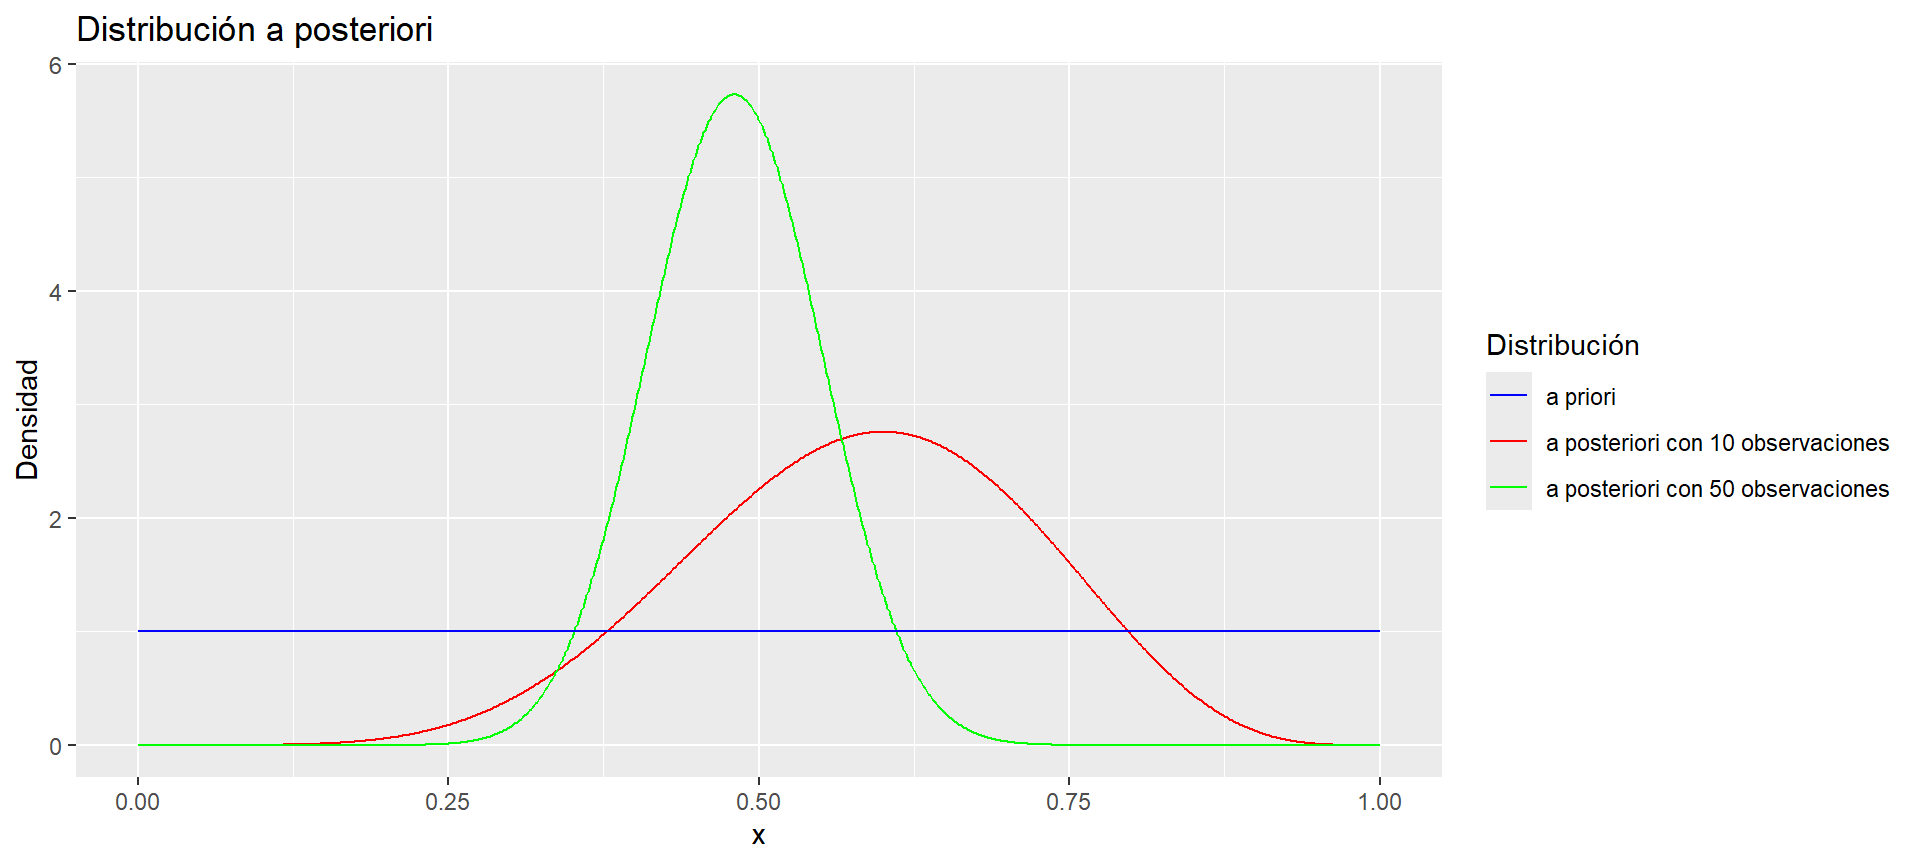
\includegraphics[width=\linewidth]{Tema 3/figures/Figure 3}
\end{minipage}
$\begin{array}{l}
    \overline{x}=20.02\\
1-\alpha=0.09\\
\alpha=0.1\\
\dfrac{\alpha}{2}=0.05\\
\left(20.2\mp 1.645 \dfrac{0.05}{\sqrt{5} }\right)=(20.02\mp 0.0367) = (19.9833, 20.0588)
\end{array}$

\subsection{Comentarios importantes}
\begin{tcolorbox}[colback=olive!5!white, colframe=olive!75!black, title=\textbf{Si $X$ no es Normal}]
\begin{itemize}[label=\textbullet]
    \item Hemos trabajado con la hipótesis de que $X$ es Normal para encontrar el estadístico pivotal $\dfrac{\overline{X}-\mu}{\sigma / \sqrt{n} }\sim \mathcal{N}(0,1)$.
    \item Si $X$ no es Normal, no podemos garantizar la confianza especificada.
    \item Sin embargo, si $n$ grande, tenemos por el Teorema Central del Límite \[
    \dfrac{\overline{X}-\mu}{\sigma / \sqrt{n} }\sim \mathcal{N}(0,1),\text{ aproximiadamente, }
    \] 
    entonces la confianza especificada no será exacta pero casi\dots
\end{itemize}
\end{tcolorbox}
\subsubsection{Factores que afectan a la precisión de la estimación}
\begin{tcolorbox}[colback=olive!5!white, colframe=olive!75!black, title=\textbf{El margen de error es $z_{1-\alpha /2}\dfrac{\sigma}{\sqrt{n} }$.}]
\begin{itemize}[label=\textbullet]
    \item $n\uparrow\longrightarrow \text{ precisión }\uparrow$
    \item $\sigma\uparrow\longrightarrow \text{ precisión }\downarrow$ 
    \item Confianza $\uparrow\longrightarrow $ precisión $\downarrow$
\end{itemize}
\end{tcolorbox}
\subsubsection{Determinación del tamaño muestral}
\begin{tcolorbox}[colback=blue!5!white, colframe=blue!75!black, title=\textbf{Contexto}]
Antes de extraer la muestra:
\begin{itemize}[label=\textbullet]
    \item Tenemos decidido el valor de $\sigma$.
    \item Tenemos decidido la confianza con la que trabajamos.
    \item Tenemos decidio el margen de error máximo $max$ que estamos dispuestos a comenter.
\end{itemize}
¿Qué tamaño de la muestra debemos escoger?
\end{tcolorbox}
Margen de error: $z_{1-\alpha /2}\dfrac{\sigma}{\sqrt{n} }\le max.\longrightarrow $ Despejamos $n$
\subsubsection{Otros modelos, estadísticos pivotales}
 \begin{tcolorbox}[colback=blue!5!white, colframe=blue!75!black, title=\textbf{$X\sim \mathcal{N}(\mu,\sigma^2)$, estimamos $\mu,\sigma$ desconocida}]
Estadístico pivotal: \[
T=\dfrac{\overline{X}-\mu}{S / \sqrt{n} }\sim t_{n-1}
\] 
\end{tcolorbox}

Debemos encontrar valores $a$ y $b$ tales que:

\begin{minipage}{0.45\textwidth}
    \includegraphics[width=\linewidth]{"Tema 3/figures/Figure 4"}
\end{minipage}$\begin{array}{l}
    P\left[ a\le \dfrac{\overline{X}-\mu}{S / \sqrt{n} }\le b \right] \\
    P\left[ -t_{n-1,1-\frac{\alpha}{2}}\le \dfrac{\overline{X}-\mu}{S / \sqrt{n} }\le t_{n-1,1-\frac{\alpha}{2} } \right] \\
    P\left[ X-t_{n-1,1-\frac{\alpha}{2} }\dfrac{S}{\sqrt{n} }\le \dfrac{\overline{X}-\mu}{S / \sqrt{n} }\le X+t_{n-1,1-\frac{\alpha}{2} }\dfrac{S}{\sqrt{n} } \right] =1-\alpha
\end{array}$

Obteniendo como I.C aleatorio a nivel $100(1-\alpha)\%$ \[
X-t_{n-1,1-\frac{\alpha}{2} }\dfrac{S}{\sqrt{n} }
\] 
\begin{tcolorbox}[colback=blue!5!white, colframe=blue!75!black, title=\textbf{$X\sim \mathcal{N}(\mu,\sigma^2)$, estimamos $\sigma^2$}]
Estadístico pivotal: \[
\dfrac{(n-1)S_n^2}{\sigma^2}\sim \chi_{n-1}^2
\] 
\end{tcolorbox}
I.C para $\sigma^2$ al nivel de confianza $(1-\alpha)100\%$ \[
T=\dfrac{(n-1)s^2}{\sigma^2}\leadsto \chi_{n-1}^2
\] 
Debemos encontrar valores $a$ y $b$ tales que: $P\left[ a\le \dfrac{(n-1)s^2}{\sigma^2}\le b \right]=1-\alpha $

\begin{minipage}{0.45\textwidth}
    \includegraphics[width=\linewidth]{"Tema 3/figures/Figure 5"}
\end{minipage}
$\begin{array}{l}
    P\left[ -\chi_{n-1,\frac{1-\alpha}{2} }^2\le \dfrac{(n-1)s^2}{\sigma^2}\le \chi_{n-1,1-\frac{\alpha}{2} }^2 \right] =1-\alpha\\
    P\left[ -\dfrac{1}{\chi_{n-1,1-\frac{\alpha}{2}}} \le  \dfrac{\sigma^2}{(n-1)s^2}\le \dfrac{1}{\chi_{n-1,1-\frac{\alpha}{2} }^2} \right] =1-\alpha\\
    P\left[ -\dfrac{(n-1)s^2}{\chi_{n-1,1-\frac{\alpha}{2} }^2}\le \sigma^2\le \dfrac{(n-1)s^2}{\chi_{n-1,1-\frac{\alpha}{2} }^2} \right] =1-\alpha
\end{array}$


\newpage

\section{Análisis de componentes principales}
\subsection{Introducción}
\begin{enumerate}[label=\arabic*)]
	\item Objetivo
\end{enumerate}
Simplificar la representación de datos multidimensionales al transformarlos en un nuevo conjunto de variables llamadas \lb{componentes principales}.
\begin{itemize}
	\item \lb{Reducción de dimensionalidad:} a veces dispondremos de muchas variables y simplemente se querrá disminuir el número de variables perdiendo la menor información posible (\lb{compresión de datos}).
	\begin{itemize}
		\item Útil en aplicaciones de almacenamiento y transmisión de información.
	\end{itemize}
	\item \lb{Visualización de datos:} al proyectar los datos en un espacio de menor dimensión, es más fácil representar gráficamente la estructura subyacente de los datos, lo que puede ayudar a identificar patrones, agrupaciones o relaciones (\lb{extracción de características}).
	\item \lb{Eliminación de multicolinealidad:} en análisis de regresión y otros contextos, la multicolinealidad (alta correlación entre variables independientes) puede ser problemática.
	\begin{itemize}
		\item En estos casos puede ayudar a reducir la multicolinealidad el \lb{transformar las variables originales} en un conjunto de variables no correlacionadas (las \lb{componentes principales}).
	\end{itemize}
\end{itemize}
\begin{itemize}[label=\color{red}\textbullet, leftmargin=*]
	\item \color{lightblue}Planteamiento desde el punto de vista teórico
\end{itemize}
La idea es \lb{resumir la información} de un \vea (v.a.) $k$-dimensional $\mathbf{X}=(X_1,\dots,X_k)'$ (recordemos que $A'$ denota la traspuesta de $A$, es decir, $\mathbf{X}$ es un vector columna) en unas \lb{pocas variables} que proporcionen la información más relevante.

Se puede dar una aproximación geométrica mediante el concepto de \lb{elipsoide de concentración}.
\begin{itemize}[label=\color{red}\textbullet, leftmargin=*]
	\item \color{lightblue}Definición
\end{itemize}
Si $\mathbf{X}$ es un vector aleatorio de dimensión $k$, media $\mu$ y su matriz de covarianzas $V=(\sigma_{i,j})$ definida positiva, se define el \lb{elipsoide de concentración} de $\mathbf{X}$ como \[ E_k=\{\mathbf{x}\in\R^k:(\mathbf{x}-\mu)'V^{-1}(\mathbf{x}-\mu)\le k+2\}. \]
En la definición del elipsoide interviene la \lb{distancia de Mahalanobis basada en la matriz $V$} entre $\mathbf{x}$ y la media $\mu$ dada por \[ d_V(\mathbf{x},\mu)=\sqrt{(\mathbf{x}-\mu)'V^{-1}(\mathbf{x}-\mu)}. \]
Esta distancia al cuadrado se puede calcular en \code{R} con \code{mahalanobis(x, mu, V)}.

Además, si $X$ es \lb{normal}, el elipsoide se puede definir a partir de las \lb{curvas de nivel de la función de densidad} ($f(x)=cte$.) ya que \[ f(x)=\dfrac{1}{\sqrt{|V|(2\pi)^k}}\exp\left(-\dfrac{1}{2}(\mathbf{x}-\mu)'V^{-1}(\mathbf{x}-\mu)\right). \]
Una parte de los individuos (puntos estarán dentro de este elipsoide).

Si queremos \lb{distinguirlos con una única variable}, parece claro que lo mejor sería proyectarlos sobre el eje mayor del elipsoide.

Por ejemplo, para una \lb{normal bivariante} \[ \mathcal{N}_2\left(\mu=\binom{0}{0},V=\begin{pmatrix}
	1 & \tfrac{1}{2}\\
	\tfrac{1}{2} & 1
\end{pmatrix}\right) \] se tiene que \[ (x_1,x_2)\begin{pmatrix}
1 & \tfrac{1}{2}\\
\tfrac{1}{2} & 1
\end{pmatrix}^{-1}\binom{x_1}{x_2}=\dfrac{4}{3}x_1^2-\dfrac{4}{3}x_1x_2+\dfrac{4}{3}x_2^2 \] por lo que el \lb{elipsoide de concentración} sería \[ \dfrac{4}{3}x_1^2-\dfrac{4}{3}x_1x_2+\dfrac{4}{3}x_2^2\le4 \]

\begin{itemize}
	\item \lb{Elipsoide de concentración} para la normal bivariante con medias 0, varianzas 1 y correlación $\dfrac{1}{2}:$
	
	\begin{lstlisting}
hc <- function(x1, x2) (4/3)*x1^ 2- (4/3)*x1*x2 + (4/3)*x2^ 2
x1 <- seq(-3, 3, length =1000)
x2 <- seq(-3, 3, length =1000)
z <- outer(x1, x2, hc)
contour(x1, x2, z, levels = 4)
title(main = "level = 4")
	\end{lstlisting}
	\begin{center}
		\includegraphics[width=0.5\linewidth]{"Temas/Imágenes/Tema 4/screenshot001"}
	\end{center}
	\item \lb{Elipsoides obtenidos con otros niveles} (circunferencias de Mahalanobis):
	\begin{lstlisting}
hc <- function(x1, x2) (4/3)*x1^ 2- (4/3)*x1*x2 + (4/3)*x2^ 2
x1 <- seq(-3, 3, length =1000)
x2 <- seq(-3, 3, length =1000)
z <- outer(x1, x2, hc)
contour(x1, x2, z, levels = c(1:6))
title(main = "level = 1, ..., 6")
	\end{lstlisting}
	\begin{center}
		\includegraphics[width=0.5\linewidth]{"Temas/Imágenes/Tema 4/screenshot002"}
	\end{center}
\end{itemize}

\begin{minipage}{0.45\textwidth}
	Si queremos \lb{reducir las dos variables a solo una}, la mejor proyección, es decir la que mejor separa los puntos (\lb{varianza máxima}), es la proporcionada por el \lb{eje principal del elipsoide} (o curvas de nivel de la normal).
	
	En este ejemplo viene dado por la recta: \[ x_2=x_1. \]
\end{minipage}\qquad\begin{minipage}{0.5\textwidth}
\begin{lstlisting}
hc <- function(x1, x2) (4/3)*x1^ 2- (4/3)*x1*x2 + (4/3)*x2^ 2
x1 <- seq(-3, 3, length =1000)
x2 <- seq(-3, 3, length =1000)
z <- outer(x1, x2, hc)
contour(x1, x2, z, levels = c(1:6))
abline(a = 0, b = 1, col = "red", lty = 2)
abline(a = 0, b = -1, col = "blue", lty = 2)
title(main = "level = 1, ..., 6")
\end{lstlisting}
\end{minipage}
\begin{flushright}
\includegraphics[width=0.5\linewidth]{"Temas/Imágenes/Tema 4/screenshot003"}
\end{flushright}
\begin{itemize}[label=\color{red}\textbullet, leftmargin=*]
	\item \color{lightblue}Objetivo
\end{itemize}
\lb{Transformar} un conjunto de $k$ variables interrelacionadas entre sí en un nuevo conjunto con un número menor de variables:
\begin{itemize}
	\item las \lb{componentes principales}
\end{itemize}
De manera que estas nuevas variables:
\begin{itemize}
	\item sean \lb{ortogonales entre sí}.
	\item capturen la \lb{mayor variabilidad} de las variables.
	\item \lb{expliquen la mayor parte de la variabilidad} de las variables originales.
\end{itemize}
\begin{itemize}[label=\color{red}\textbullet, leftmargin=*]
	\item \color{lightblue}Planteamiento teórico
\end{itemize}
Supongamos que $\mathbf{X}=(X_1,\dots,X_k)'$ es un \vea $k$-dimensional con vector de medias $\mu$ y matriz de covarianzas $V$ \lb{semidefinida positiva}.

Entonces la \lb{primera componente principal} será la \va unidimensional \[ Y_1=a_1X_1+\cdots+a_kX_k \] con $a_1^2+\cdots+a_k^2=1$ cuya \lb{varianza es máxima}.
\begin{itemize}
	\item Si no se normaliza la combinación lineal, la variable $Y_1$ puede tener varianza tan grande como queramos.
	\item Geométricamente, hacemos un cambio de variable (primer eje) para que la dispersión sea máxima y la normalización equivale a mantener la escala original (proyectar).
\end{itemize}
El problema puede expresarse de la forma siguiente: \[ \begin{rcases}
	\max&\var(a'\mathbf{X})\\
	\text{s.a.} & \mathbf{a'a}=1
\end{rcases} \] donde $\mathbf{a}=(a_1,\dots,a_k)'\in\R^k$.

Una vez calculada una primera componente principal $Y_1$, la \lb{segunda componente principal} $Y_2$ debe verificar $\cov(Y_1,Y_2)=0$ (no debe contener información ya incluida en $Y_1$) y debe tener la \lb{varianza máxima}, es decir, \[ \begin{rcases}
	\max & \var(\mathbf{a'X})\\
	\text{s.a.} & \mathbf{a'a}=1\\
	&\cov(Y_1,\mathbf{a'X})=0
\end{rcases} \]
Así, sucesivamente, por inducción, se definen las \lb{siguientes componentes principales} $(Y_j)$ como la (una) solución de 
\[ \begin{rcases}
	\max & \var(\mathbf{a'X})\\
	\text{s.a.} & \mathbf{a'a}=1\\
	&\cov(Y_1,\mathbf{a'X})=0,\quad i=1,\dots,j-1
\end{rcases} \]
\begin{itemize}[label=\color{lightblue}\textbullet]
	\item La solución general viene dada en el teorema siguiente que prueba la \lb{existencia de las (unas) componentes principales} y muestra \lb{cómo calcularlas}.
	\item Además, se demuestra que las componentes principales \lb{no son únicas} (puede haber más soluciones).
\end{itemize}
\begin{itemize}[label=\color{red}\textbullet, leftmargin=*]
	\item \color{lightblue}Teorema de existencia
\end{itemize}
Si $\mathbf{X}$ es un \vea $k$-dimensional con matriz de covarianzas $V$ \lb{definida positiva}, las (unas) \lb{componentes principales} se obtienen como \[ \mathbf{Y}=(Y_1,\dots,Y_k)'=T'\mathbf{X}=\begin{pmatrix}
	t_{1,1} & \cdots & t_{k,1} \\
	\cdots & \cdots & \cdots \\
	t_{1,k} & \cdots & t_{k,k}
\end{pmatrix}\begin{pmatrix}
X_1\\
\cdots\\
X_k
\end{pmatrix}, \] donde $T$ es una \lb{matriz ortogonal} $(T'T=TT'=I)$ tal que \[ T'VT=D=\mathrm{diag}(\lambda_1,\dots,\lambda_k) \]con $\lambda_1\ge\lambda_2\ge\cdots\ge\lambda_k>0$.
\begin{itemize}[label=\color{red}\textbullet, leftmargin=*]
	\item \color{lightblue}Demostración
\end{itemize}
Como $V$ es una matriz \lb{simétrica} y \lb{definida positiva}, existe una matriz $T=(t_{i,j})$ \lb{ortogonal} $(T'T=TT'=I)$ tal que \[ T'VT=D=\mathrm{diag}(\lambda_1,\dots,\lambda_k) \] con los valores propios verificando $\lambda_1\ge\lambda_2\ge\cdots\ge\lambda_k>0$.

De esta forma, si \[ \mathbf{Y}=(Y_1,\dots,Y_k)'=T'\mathbf{X}=\begin{pmatrix}
	t_{1,1} & \cdots & t_{k,1} \\
	\cdots & \cdots & \cdots \\
	t_{1,k} & \cdots & t_{k,k}
\end{pmatrix}\begin{pmatrix}
	X_1\\
	\cdots\\
	X_k
\end{pmatrix} \] entonces $Y_1,\dots,Y_k$ verifican que \[ \cov(\mathbf{Y})=\cov(T'\mathbf{X})=E[T'(\mathbf{X-\mu})(\mathbf{X}-\mu)'T]=T'VT=D, \]lo que indica que $\cov(Y_i,Y_j)=0$ para $i\neq j$ y $\var(Y_j)=\lambda_j$.

Para comprobar que $Y_1$ es una primera componente principal, supongamos que $\mathbf{a'X}$ es una combinación lineal con $\mathbf{a'a}=1$.

Las columnas de la matriz $T$ corresponden a los vectores propios $\mathbf{t}_i$ asociados a los autovalores $\lambda_i,T=(\mathbf{t}_1|\cdots|\mathbf{t}_k)$, y como los vectores propios son una base, existirán $c_1,\dots,c_k$ números reales tales que \[ \mathbf{a}=c_1\mathbf{t}_1+\cdots+c_k\mathbf{t}_k=\sum_{i=1}^{k}c_i\mathbf{t}_i. \]
Con lo que 
\begin{align*}
	\var(\mathbf{a'X})&=E[\mathbf{a'(X-\mu)(X-\mu)'a}]=\mathbf{a}'\cov(\mathbf{X})\mathbf{a}=\mathbf{a'}V\mathbf{a}\\
	&=\left(\sum_{i=1}^{k}c_i\mathbf{t}_i'\right)V\left(\sum_{i=1}^{k}c_i\mathbf{t}_i\right)=\left(\sum_{i=1}^{k}c_i\mathbf{t}_i'\right)\left(\sum_{j=1}^{k}c_jV\mathbf{t}_j\right)\\
	&=\left(\sum_{i=1}^{k}c_i\mathbf{t}_i'\right)\left(\sum_{j=1}^{k}c_j\lambda_j\mathbf{t}_j\right)=\sum_{i,j}c_ic_j\lambda_j\mathbf{t}_i'\mathbf{t}_j=\sum_{i=1}^{k}c_i^2\lambda_i
\end{align*}
Y, como \[ \mathbf{a'a}=\left(\sum_{i=1}^{k}c_i\mathbf{t}_i'\right)\left(\sum_{j=1}^{k}c_j\mathbf{t}_j\right)=\sum_{i,j}c_ic_j\mathbf{t}_i'\mathbf{t}_j=\sum_{i=1}^{k}c_i^2=\mathbf{c'c}=1, \] con $\mathbf{c}=(c_1,\dots,c_k)'$, la varianza será máxima si $x_1^2=1,c_2=0,\dots,c_k=0$ ya que \[ \var(\pm\mathbf{t}_1'\mathbf{X})=\lambda_1=\mathbf{c'c}\lambda_1=\sum_{i=1}^{k}c_i^2\lambda_1\ge\sum_{i=1}^{k}c_i^2\lambda_i=\var(\mathbf{a'X}), \]para todo $\mathbf{a}$ tal que $\mathbf{a'a}=1$, es decir, $Y_1=\pm \mathbf{t}_1'\mathbf{X}$ es una primera componente principal (puede haber otras soluciones si $\lambda_1=\lambda_2$).

Por inducción, supongamos que $Y_1=\mathbf{t}_1'\mathbf{X},\dots,Y_{j-1}\mathbf{X}$ son las primeras ($j-1$) componentes principales.

Y veamos que $Y_j=\mathbf{t}_j'\mathbf{X}$ es la (una) solución de \[ \begin{rcases}
	\max & \var(\mathbf{a'X})\\
	\text{s.a.} & \mathbf{a'a}=1\\
	&\cov(Y_1,\mathbf{a'X})=0,\quad i=1,\dots,j-1
\end{rcases} \]
Como se debe verificar \begin{align*}
	\cov(\mathbf{a'X},Y_i) & = \cov(\mathbf{a'X},\mathbf{t}_i'\mathbf{X})=E[\mathbf{a'(X-\mu)(X-\mu)'t}_i]=\mathbf{a}'\cov(\mathbf{X})\mathbf{t}_i\\
	&=\mathbf{a'}V\mathbf{t}_i=\mathbf{a'\lambda}_i\mathbf{t}_i=\lambda_i\mathbf{a't}_i=\lambda_i\left(\sum_sc_s\mathbf{t}_s'\right)\mathbf{t}_i=\lambda_ic_i=0
\end{align*} para $i=1,\dots,j-1,\:\lambda_i>0$, se tiene $c_1=\cdots=c_{j-1}=0$.

Entonces, la varianza será máxima si $c_j=1$ y $c_i=0$ para $i>j$, ya que \[ \var(\pm\mathbf{t}_j'\mathbf{X})=\lambda_j=\mathbf{c'c}\lambda_j=\sum_{i=j}^{k}c_i^2\lambda_j\ge\sum_{i=j}^{k}c_i^2\lambda_i=\var(\mathbf{a'X}), \] para todo $\mathbf{a}$ tal que $\mathbf{a'a}=1$ y $\cov(\mathbf{a'X}, Y_i)=0,\:i=1,\dots,j-1$, es decir, $Y_j=\pm\mathbf{t}_j'\mathbf{X}$ es una componente principal $j$-ésima (no necesariamente la única).

\begin{itemize}[label=\color{red}\textbullet, leftmargin=*]
	\item \color{lightblue}Corolario
\end{itemize}
Si $\lambda_1>\lambda_2>\cdots>\lambda_k$, entonces las componentes principales son únicas salvo digno.
\begin{itemize}[label=\color{red}\textbullet, leftmargin=*]
	\item \color{lightblue}Observación
\end{itemize}
Nótese que la componente principal $j$-ésima se obtiene multiplicando la fila $j$-ésima de $T'$ (la columna $j$-ésima de $T$) por $\mathbf{X}$, es decir, \[ Y_j=\mathbf{t}_j'\mathbf{X} \]donde $\mathbf{t}_j'=(t_{1,j},\dots,t_{k,j})$ es un vector propio unitario correspondiente al $j$-ésimo valor propio (vectores columna de $T$).

Además, $\var(Y_j)=\lambda_j$, y \[ \mathrm{traza}(V)=\sum_{j=1}^{k}\sigma_{j,j}=\sum_{j=1}^{k}\var(X_j)=\sum_{j=1}^{k}\var(Y_j)=\sum_{j=1}^{k}\lambda_j \](las matrices semejantes tienen las trazas iguales), es decir, la \lb{variabilidad} (información) de las variables originales es igual a la suma de las variabilidades de las componentes principales.

La \lb{cantidad de información} (\%) contenida en cada componente será \[ I_j=100\dfrac{\lambda_j}{\displaystyle\sum_{i=1}^{k}\lambda_i}\%. \]
Por esto, la \lb{traza} se usar como una medida unidimensional de la dispersión de una variable $k$-dimensional.

La otra medida es el \lb{determinante} de $V$ para el que también se verifica: \[ |V|=\lambda_1\cdots\lambda_k=|\cov(\mathbf{Y})| \]
\begin{itemize}[label=\color{red}\textbullet, leftmargin=*]
	\item \color{lightblue}Observación
\end{itemize}
Otros autores llaman componentes principales a \[ \mathbf{Y}=T'(\mathbf{X-\mu}) \] con lo que, además, se consigue que sean centradas ($E[Y_j]=0$),
\begin{itemize}
	\item \lb{compronentes principales centradas}
\end{itemize}
También se pueden definir las \lb{componentes principales estandarizadas} \[ Z_j=\mathbf{t}_j'(\mathbf{X-\mu})\lambda_j^{-\frac{1}{2}} \] $(\mathbf{Z}=D^{-\frac{1}{2}}T'(\mathbf{X-\mu}))$ que además de ser centradas tendrán varianza 1.

Cuando hay \lb{valores propios iguales a cero} ($V$ es \lb{semidefinida positiva}) no suelen considerarse sus correspondientes componentes principales (degeneradas) y se puede conservar toda la información en las componentes principales de valores propios distintos de cero.

En este caso hay \lb{variables} que pueden obtenerse como \lb{combinación lineal de las restantes} (aunque no siempre pueden eliminarse del análisis).

Geométricamente, las \lb{componentes principales} se corresponden con los \lb{ejes principales del elipsoide de concentración}.

Como $\mathbf{Y}=T'\mathbf{X}$, podemos interpretar las componentes en función de los pesos que tengan en ellas las variables originales.

Si ponemos $\mathbf{X}$ en función de $\mathbf{Y}$ como $\mathbf{X}=T\mathbf{Y}$, entonces las variables originales se pueden interpretar en función de las componentes principales e incluso, podemos representar aproximadamente, las variables originales usando las dos (tres) primeras componentes.
\begin{itemize}[label=\color{red}\textbullet, leftmargin=*]
	\item \color{lightblue}Caso de normalidad
\end{itemize}
Si la población $\mathbf{X}$ es \lb{normal}, entonces las \lb{componentes principales} son \lb{normales} e \lb{independientes entre sí}, ya que en estas poblaciones equivalen los conceptos de independencia e incorrelación (independencia lineal) y $\mathbf{Z}$ será una normal estándar multivariante ($\mathcal{N}_k(0,I)$).
\begin{itemize}[label=\color{red}\textbullet, leftmargin=*]
	\item \color{lightblue}Proposición
\end{itemize}
Si $\mathbf{Y}$ son las \lb{componentes principales} obtenidas a partir de $\mathbf{X}$, entonces $\mathbf{X}$ es \lb{normal multivariante} si, y sólo si $Y_1,\dots,Y_k$ son \lb{independientes} y \lb{normales univariantes} para todo $j=1,\dots,k$.
\begin{itemize}[label=\color{red}\textbullet, leftmargin=*]
	\item \color{lightblue}Demostración.
\end{itemize}
La demostración es inmediata.

Esta propiedad puede ser utilizada para estudiar la normalidad multivariante a partir de un test de normalidad univariante sobre las componentes principales.

Incluso si la normal multivariante no es de rango completo ($V$ no es definida positiva), puede utilizarse con con las $m$ primeras componentes con valores propios distintos de cero (las otras serán degeneradas) coincidiendo $m$ con el rango de $V$.

\Ej

Para el \vea normal de media $\mu=(0,0)$ y matriz de covarianzas $V=\begin{pmatrix}
	1 & \tfrac{1}{2}\\
	\tfrac{1}{2} & 1
\end{pmatrix}$

\hspace{1cm}

\begin{lstlisting}
library("mvtnorm")
f <- function(x1, x2) dmvnorm(data.frame(x1, x2), mu, V)
V <- matrix(c(1, 1/2,
1/2, 1), nrow = 2, ncol = 2, byrow = TRUE)
mu <- c(0, 0)
x1 <- seq(-3, 3, length = 50)
x2 <- seq(-3, 3, length = 50)
z <- outer(x1, x2, f)
persp(x1, x2, z, xlab = 'x1', ylab = 'x2', zlab = 'f(x1, x2)', col = 'orange', main = "Función de densidad")
\end{lstlisting}
\begin{center}
	\includegraphics[width=0.6\linewidth]{"Temas/Imágenes/Tema 4/screenshot004"}
\end{center}

\pagebreak

\begin{lstlisting}
#Se fija la semilla para la generación aleatoria
set.seed(123)
d <- rmvnorm(50, mu, V)
plot(d, xlab = "X1", ylab = "X2", pch = 20, xlim = c(-3, 3), ylim = c(-3, 3), main = "Elipsoide de concentración")
hc <- function(x1, x2) (4/3)*x1^ 2 - (4/3)*x1*x2 + (4/3)*x2^ 2
x1 <- seq(-3, 3, length = 1000)
x2 <- seq(-3, 3, length = 1000)
z <- outer(x1, x2, hc)
contour(x1, x2, z, levels = 4, add = T, col = 'red')
\end{lstlisting}
\begin{center}
	\includegraphics[width=0.6\linewidth]{"Temas/Imágenes/Tema 4/screenshot005"}
\end{center}
Sus componentes principales se calcularán diagonalizando $V$ mediante \[ \left|V-\lambda I\right|=\begin{vmatrix}
	1-\lambda & 0.5\\
	0.5 & 1-\lambda
\end{vmatrix}=1-2\lambda+\lambda^2-\dfrac{1}{4}=0 \] que tiene soluciones \[ \lambda=\dfrac{2\pm\sqrt{4-4(1-\frac{1}{4})}}{2}=1\pm0.5, \]$\lambda_1=1.5$ y $\lambda_2=0.5$.

Y la \lb{primera componente} se obtendrá resolviendo $V\mathbf{v}=\lambda\mathbf{v}$ \[ \begin{pmatrix}
	1 & 0.5\\
	0.5 & 1
\end{pmatrix}\begin{pmatrix}
x_1\\
x_2
\end{pmatrix}=1.5\begin{pmatrix}
x_1\\
x_2
\end{pmatrix}\xRightarrow{\qquad}\begin{pmatrix}
-0.5x_1+0.5x_2\\
0.5x_1-0.5x_2
\end{pmatrix}=\begin{pmatrix}
0\\
0
\end{pmatrix} \]lo que da $x_1=x_2$, es decir, sus vectores propios son de la forma $\mathbf{v}=\alpha(1,1)'$.

Como usamos vectores normalizados (de norma 1), una primera componente valdrá \[ Y_1=\left(\dfrac{1}{\sqrt{2}},\dfrac{1}{\sqrt{2}}\right)\dbinom{X_1}{X_2}=\dfrac{X_1+X_2}{\sqrt{2}} \]y su varianza es $\lambda_1=1.5$.

Análogamente, la segunda valdrá $Y_2=\dfrac{X_1-X_2}{\sqrt{2}}$ (ya que tiene que ser perpendicular a la primera) y tendrá varianza $\lambda_2=0.5$.

Es decir, tenemos \[ \begin{array}{l}
	Y_1=\dfrac{X_1+X_2}{\sqrt{2}}\\
	Y_2=\dfrac{X_1-X_2}{\sqrt{2}}\\
\end{array} \]por lo que \[ \mathbf{Y}=T'\mathbf{X}=\begin{pmatrix}
\frac{1}{\sqrt{2}} & \frac{1}{\sqrt{2}}\\
\frac{1}{\sqrt{2}} & -\frac{1}{\sqrt{2}}\\
\end{pmatrix}\begin{pmatrix}
X_1\\
X_2
\end{pmatrix}. \]
\lb{Varianza total explicada} por cada componente:
\begin{itemize}
	\item La primera componente explicará un 75\% de la varianza total: \[ I_1=100\dfrac{\lambda_1}{\lambda_1+\lambda_2}\%=75\%. \]
	\item La segunda un 25\% de la varianza total: \[ I_2=100\dfrac{\lambda_2}{\lambda_1+\lambda_2}\%=25\%. \]
\end{itemize}
Como las varianzas iniciales son iguales, ambas tienen igual peso en las componentes con distinto signo en el caso de la segunda de ellas.

Aunque las varianzas iniciales sean todas iguales (1) las componentes principales tienen varianzas (en general) distintas.

Si $X_1$ fuese el peso de una persona y $X_2$ su altura (estandarizadas).
\begin{itemize}
	\item La primera componente se podría interpretar como lo \lb{grande} que es dicha persona.
	\item Mientras que la segunda estará relacionada con su \lb{constitución} ($Y_2$ grande significaría mucho peso y poca altura, es decir, complexión fuerte).
\end{itemize}
Despejando, se tiene \[ \begin{array}{l}
	X_1=\dfrac{Y_1+Y_2}{\sqrt{2}}\\
	X_2=\dfrac{Y_1-Y_2}{\sqrt{2}}\\
\end{array} \] lo que nos permite representar las variables $X_1,\:X_2$ en función de las componentes $Y_1,\:Y_2$.
\begin{itemize}
	\item $Y_1$ aumenta si lo hacen $X_1$ y $X_2$.
	\item $Y_2$ aumenta si aumenta $X_1$ y disminuye $X_2$.
	\item Estas relaciones servirán para interpretar (dar significado) a las componentes principales.
\end{itemize}
\subsection{¿Cómo realizamos estos cálculo en \textbf{\texttt{R}}?}
En primer lugar definimos e introducimos $V$
\begin{lstlisting}
V <- matrix(c(1, 1/2, 1/2, 1), nrow = 2, ncol = 2, byrow = TRUE)
V
\end{lstlisting}
\begin{verbatim}
##      [,1] [,2]
## [1,]  1.0  0.5
## [2,]  0.5  1.0
\end{verbatim}
Calculamos los valores y vectores propios:
\begin{lstlisting}
eigen(V)$values; eigen(V)$vectors
\end{lstlisting}
\begin{verbatim}
## [1] 1.5 0.5
##           [,1]       [,2]
## [1,] 0.7071068 -0.7071068
## [2,] 0.7071068  0.7071068
\end{verbatim}
Podemos guardar la matriz $T$ de vectores propios:
\begin{lstlisting}[mathescape=false]
T <- eigen(V)$vectors
\end{lstlisting}
Los vectores normalizados aparecen en las columnas de $T$. Podemos comprobar que $T$ es una matriz ortogonal:
\begin{lstlisting}
t(T) %*% T
\end{lstlisting}
\begin{verbatim}
##      [,1] [,2]
## [1,]    1    0
## [2,]    0    1
\end{verbatim}
donde \code{t(A)} es la traspuesta de \code{A} y \code{A \%*\% B} es el producto de las matrices \code{A} y \code{B} en \code{R}.

Podemos comprobar que $T$ diagonaliza a $V$:
\begin{lstlisting}
t(T) %*% V %*% T
\end{lstlisting}
\begin{verbatim}
##      [,1] [,2]
## [1,]  1.5  0.0
## [2,]  0.0  0.5
\end{verbatim}
lo que nos dará la matriz diagonal con los valores 1.5 y 0.5 en la diagonal.

Como $\mathbf{Y}=T'\mathbf{X}$, las componentes principales serán \[ \begin{array}{l}
	Y_1=0.7071068X_1+0.7071068X_2=\dfrac{X_1+X_2}{\sqrt{2}}\\
	Y_2=-0.7071068X_1+0.7071068X_2=-\dfrac{X_1+X_2}{\sqrt{2}}\\
\end{array} \]
Para calcular las informaciones contenidas en cada una (en tanto por 100) haremos:
\begin{lstlisting}
100*eigen(V)$values/sum(eigen(V)$values)
\end{lstlisting}
\begin{verbatim}
## [1] 75 25
\end{verbatim}
obteniendo el 75\% y el 25\%
\subsection{Desigualdades}
Si $Z$ es una variable aleatoria no negativa con media finita $E[Z]$ y $\epsilon>0$, entonces \[ \epsilon Pr[Z\ge\epsilon]=\epsilon\int_{[\epsilon,\infty)}\mathrm{d}F_Z(x)\le\int_{[\epsilon,\infty)}x\mathrm{d}F_Z(x)\le\int_{[0,\infty)}x\mathrm{d}F_Z(x)=E(Z) \] (donde $F_Z(x)=Pr[Z\le x]$ es su función de distribución), es decir \[ Pr[Z\ge \epsilon]\le\dfrac{E[Z]}{\epsilon}. \]

$\bboxed{E\left[\dfrac{(X-\mu)^2}{\sigma^2}\right]=\dfrac{1}{\sigma^2}E[(X-\mu)^2]=\dfrac{\sigma^2}{\sigma^2}=1}$

Si $X$ es una variable aleatoria con media finita $\mu=E[X]$ y varianza $\sigma^2=\var(X)>0$, entonces tomando $Z=\dfrac{(X-\mu)^2}{\sigma^2}\ge0$ y aplicando la desigualdad de Markov, tenemos \[ Pr\left[\dfrac{(X-\mu)^2}{\sigma^2}\ge\epsilon\right]\le\dfrac{1}{\epsilon} \]para todo $\epsilon>0$.
\subsubsection{Desigualdad de Chebyshev}
También se puede escribir como \[ Pr[(X-\mu)^2<\epsilon\sigma^2]\ge1-\dfrac{1}{\epsilon}, \] o como \[ Pr[|X-\mu|<r]\ge1-\dfrac{\sigma^2}{r^2}, \] para todo $r>0$.
\subsubsection{Desigualdad de Chebyshev multivariante}
Sea $\mathbf{X}=(X_1,\dots,X_k)'$ un \vea con vector de medias finito $\mu=E(\mathbf{X})$ y matriz de covarianzas definida positiva $V$, entonces \[ Pr[(\mathbf{X}-\mu)'V^{-1}(\mathbf{X}-\mu)\ge\epsilon]\le\dfrac{k}{\epsilon} \]para todo $\epsilon>0$.
\begin{itemize}[label=\color{red}\textbullet, leftmargin=*]
	\item \color{lightblue}Consecuencias
\end{itemize}
La desigualdad también se puede escribir como \[ Pr[(\mathbf{X}-\mu)'V^{-1}(\mathbf{X}-\mu)<\epsilon]\ge1-\dfrac{k}{\epsilon}, \] para todo $\epsilon>0$.

En particular, para el elipsoide de concentración \[ E_k=\{x\in\R^k:(\mathbf{X}-\mu)V^{-1}(\mathbf{X}-\mu)\le k+2\}, \] obtenemos \[ Pr[\mathbf{X}\in E_k]\ge1-\dfrac{k}{k+2}=\dfrac{2}{k+2}. \]
Para obtener regiones con más datos podemos tomar $\epsilon=ck$, resultando \[ Pr[(\mathbf{X}-\mu)'V^{-1}(\mathbf{X}-\mu)<ck]\ge1-\dfrac{k}{\epsilon}=1-\dfrac{1}{c}=\dfrac{c-1}{c}. \]
La \va no negativa $Z=(\mathbf{X}-\mu)'V^{-1}(\mathbf{X}-\mu)$ se puede escribir como \[ (\mathbf{X}-\mu)'TD^{-1}T'(\mathbf{X}-\mu)=\left[D^{-\frac{1}{2}}T'(\mathbf{X}-\mu)\right]'[D^{-\frac{1}{2}}T'(\mathbf{X}-\mu)]=\mathbf{Z'Z}, \] donde $\mathbf{Z}=D^{-\frac{1}{2}}T'(\mathbf{X}-\mu)\:(\mathbf{Z}=(Z_1,\dots,Z_k)')$.

Si $X$ es \lb{normal}, entonces $Z_1,\dots,Z_k$ son normales estándar independientes y \[ Z=\sum_{i=1}^{k}Z_i^2 \]sigue una \lb{distribución chi-cuadrado} con $k$ grados de libertad (ya que es la suma de $k$ normales $\mathcal{N}(0,1)$ independientes).
\subsection{Propiedades}
\begin{itemize}[label=\color{red}\textbullet, leftmargin=*]
	\item \color{lightblue}Proposición
\end{itemize}
Si $\mathbf{Y}$ son las componentes principales obtenidas a partir de $\mathbf{X}$, entonces \[ \begin{array}{l}
	\cov(\mathbf{X,Y})=TD\\
	\corr(\mathbf{X,Y})=\mathrm{diag}(V)^{-\frac{1}{2}}TD^{\frac{1}{2}}
\end{array} \] donde $\mathrm{diag}(V)=\mathrm{diag}(\sigma_1^2,\dots,\sigma_k^2)$.
\begin{itemize}[label=\color{red}\textbullet, leftmargin=*]
	\item \color{lightblue}Demostración
\end{itemize}
En primer lugar señalaremos que \[ \cov(\mathbf{X,Y})=\cov(\mathbf{X},T'\mathbf{X})=VT \] y, como $T'VT=D$ y $T$ es ortogonal, entonces $VT=TD$ y $\cov(\mathbf{X,Y})=TD$.

Por otro lado se tiene que como \[ \corr(X_i,Y_j)=\dfrac{\cov(X_i,Y_j)}{\sigma_i\lambda_j^{\frac{1}{2}}}, \]entonces \[ \corr(\mathbf{X,Y})=\mathrm{diag}(V)^{-\frac{1}{2}}\cov(\mathbf{X,Y})D^{-\frac{1}{2}} \]y\[ \corr(\mathbf{X,Y})=\mathrm{diag}(V)^{-\frac{1}{2}}TDD^{-\frac{1}{2}}=\mathrm{diag}(V)^{-\frac{1}{2}}TD^{\frac{1}{2}} \]
\begin{itemize}[label=\color{red}\textbullet, leftmargin=*]
	\item \color{lightblue}Corolario
\end{itemize}
En las condiciones de la proposición anterior se tiene: \[ \begin{array}{l}
	\cov(X_i,Y_j)=t_{i,j}\lambda_j\\
	\corr(X_i,Y_j)=\dfrac{t_{i,j}}{\sigma_i}\lambda_j^{\frac{1}{2}}
\end{array} \] para todo $i,j$.
\begin{itemize}[label=\color{red}\textbullet, leftmargin=*]
	\item \color{lightblue}Definición
\end{itemize}
Se denomina \lb{matriz de saturaciones} a \[ A=\corr(\mathbf{X,Y}). \]
\Ej

Para el \vea normal de media $\mu=(0,0)$ y matriz de covarianzas $V=\begin{pmatrix}
	1 & \tfrac{1}{2}\\
	\tfrac{1}{2} & 1
\end{pmatrix}$, se obtiene \[ T=(\mathbf{t}_1|\mathbf{t}_2)=\begin{pmatrix}
\frac{1}{\sqrt{2}} & \frac{1}{\sqrt{2}}\\
\frac{1}{\sqrt{2}} & -\frac{1}{\sqrt{2}}\\
\end{pmatrix},\quad D=\begin{pmatrix}
\lambda_1 & 0\\
0 & \lambda_2
\end{pmatrix}=\begin{pmatrix}
1.5 & 0\\
0 & 0.5
\end{pmatrix} \]por lo que la matriz de saturaciones valdrá: \[ A=\mathrm{diag}(V)^{-\frac{1}{2}}TD^{\frac{1}{2}}=\dfrac{1}{2}\begin{pmatrix}
\sqrt{3} & 1\\
\sqrt{3} & -1\\
\end{pmatrix}=\begin{pmatrix}
0.86603 & 0.5\\
0.86603 & -0.5\\
\end{pmatrix} \]

Nótese que:
\begin{itemize}
	\item La primera componente explica un 75\% (0.866\$\^\,2 \$ 100) de las variables $X_1$ y $X_2$.
	\item Mientras que la segunda solo un 25\%.
\end{itemize}
Las saturaciones y sus caudrados suelen representarse en tablas de la forma siguiente:
\[ \begin{array}{c|c|c}
	a_{i,j}=\corr(X_i,Y_j) & Y_1 & Y_2\\ \hline
	X_1 & 0.866 & 0.5\\ \hline
	X_2 & 0.866 & -0.5\\ \hline
\end{array}\qquad\begin{array}{c|c|c|c}
a_{i,j} & Y_1 & Y_2 & \text{Total}\\ \hline
X_1 & 0.75 & 0.25 & 1\\ \hline
X_2 & 0.75 & 0.25 & 1\\ \hline
\end{array} \] lo que nos puede ayudar a \lb{interceptar} las componentes principales.

Las saturaciones también se pueden representar gráficamente.

Aunque en este ejemplo, las saturaciones con las distintas variables coincidan, esto no siempre es así, y tendremos variables mejor explicadas por las componentes elegidas que otras.
\begin{itemize}[label=\color{red}\textbullet, leftmargin=*]
	\item \color{lightblue}Proposición
\end{itemize}
Si $A$ es la matriz de saturaciones, entonces \[ AA'=\corr(\mathbf{X}). \]
También es interesante calcular las correlaciones múltiples entre cada variable original con el grupo de las $p$ primeras componentes principales elegidas $(p\le k)$.
\begin{itemize}
	\item Para medir el máximo que podemos explicar de cada variable original a partir de combinaciones lineales de esas componentes principales.
\end{itemize}
\begin{itemize}[label=\color{red}\textbullet, leftmargin=*]
	\item \color{lightblue}Proposición
\end{itemize}
Si $\mathbf{Y}$ son las componentes principales obtenidas a partir de $\mathbf{X}$, entonces \[ \corr^2(X_i,(Y_1,\dots,Y_p))=\sum_{j=1}^{p}\corr^2(X_i,Y_j)=\dfrac{1}{\sigma_{i,i}}\sum_{j=1}^{p}t_{i,j}^2\lambda_j=\sum_{j=1}^{p}a_{i,j}^2. \]
La demostración es inmediata ya que las componentes son incorreladas entre sí.
\begin{itemize}[label=\color{red}\textbullet, leftmargin=*]
	\item \color{lightblue}Definición
\end{itemize}
A estas correlaciones se las suele denominar \lb{comunalidades} \[ c_i=\corr^2(X_i,(Y_1,\dots,Y_p)) \]y se suelen representar en la tabla de las saturaciones al cuadrado (como totales de las filas).

Además, el máximo de la correlación se obtiene con la combinación lineal $\alpha_i'(Y_1,\dots,Y_p)'$ con \[ \alpha_i=\lambda V_{2,2}^{-1}v_{1,2}=\lambda\begin{pmatrix}
	\lambda_1^{-1} & \cdots & 0\\
	\cdots & \cdots & \cdots\\
	0 & \cdots & \lambda_p^{-1}
\end{pmatrix}\begin{pmatrix}
t_{i,1}\lambda_1\\
\cdots\\
t_{i,p}\lambda_p
\end{pmatrix}=\lambda\begin{pmatrix}
t_{i,1}\\
\cdots\\
t_{i,p}
\end{pmatrix}. \]
Es decir, si tenemos que obtener $\mathbf{X}$ en función de las $p$ primeras componentes principales, lo haremos a partir de la relación $\mathbf{X}=T\mathbf{Y}$ eliminando el resto de las componentes.

Lógicamente, si $p=k$, se obtiene $\alpha_i'(Y_1,\dots,Y_p)=\lambda X_i$ y \[ \corr^2(X_i,(Y_1,\dots,Y_k))=\sum_{j=1}^{k}\corr^2(X_i,Y_j)=\dfrac{1}{\sigma_{i,i}}\sum_{j=1}^{k}t_{i,j}^2\lambda_j=1. \]
Recíprocamente, la información contenida en la componente principal $j$-ésima vale: \[ \lambda_j=\lambda_j\sum_{i=1}^{k}t_{i,j}^2=\sum_{i=1}^{k}\sigma_{i,i}\dfrac{1}{\sigma_{i,i}}t_{i,j}^2\lambda_j=\sum_{i=1}^{k}\sigma_{i,i}\corr^2(X_i,Y_j), \] ya que $\sum_{i=1}^{k}t_{i,j}^2=1$ es el módulo al cuadrado del vector propio $\mathbf{t}_j$ (columnas de $T$).

Y la información (variación) total contenida en las $p$ primeras componentes principales vale: \[ \sum_{j=1}^{p}\lambda_j=\sum_{j=1}^{p}\sum_{i=1}^{k}\sigma_{i,i}\corr^2(X_i,Y_j)=\sum_{i=1}^{k}\sigma_{i,i}\corr^2(X_i,(Y_1,\dots,Y_p))=\sum_{i=1}^{k}c_i\sigma_i^2. \]
Si todas las varianzas son 1, la información total $\sum_{j=1}^{p}\lambda_j$ será la suma de las comunalidades, es decir, la suma de la información que se tiene de cada variable original.
\begin{itemize}
	\item Si $p=k$, entonces $c_i=1$ y se tiene \[ \sum_{j=1}^{p}\lambda_j=\sum_{j=1}^{p}\sigma_i^2. \]
\end{itemize}
\begin{itemize}[label=\color{red}\textbullet, leftmargin=*]
	\item \color{lightblue}Seguimos con el ejemplo \dots
\end{itemize}
En el ejemplo anterior obtuvimos que: \[ \begin{array}{c|c|c|c}
	a_{i,j} & Y_1 & Y_2 & \text{Total}\\ \hline
	X_1 & 0.75 & 0.25 & 1\\ \hline
	X_2 & 0.75 & 0.25 & 1\\ \hline
	\text{Total} & 1.5 & 0.25 & 2
\end{array} \]donde:
\begin{itemize}
	\item Si $p=1$, se tiene que $\lambda_1=\dfrac{3}{2}=0.75+0.75$.
	\item Si $p=2$, se tiene que $\lambda_1+\lambda_2=\dfrac{3}{2}+\dfrac{1}{2}=2=1+1=\sigma_1^2+\sigma_2^2$.
\end{itemize}
\subsection{Cálculo a partir de la matriz de correlaciones}
Cuando se estudian variables en las que se usan unidades diferentes o queremos que éstas no sean significativas (todas las variables sean iguales a priori), las componentes principales suelen calcularse a partir de la \lb{matriz de correlaciones} \[ \Pi=(\rho_{i,j}) \]con $\rho_{i,j}=\dfrac{\sigma_{i,j}}{\sigma_i\sigma_j}$.

Esto equivale a considerar desde el principio las variables estandarizadas \[ Z_i=\dfrac{X_i-\mu_i}{\sigma_i} \](se igualan las varianzas a 1).

Usando el teorema principal, se obtienen las componentes \[ \begin{array}{c}
	\mathbf{\tilde{Y}}=\tilde{T}'\mathbf{Z}=\tilde{T}'\mathrm{diag}(V)^{-\frac{1}{2}}(\mathbf{X-\mu})\\
	\tilde{Y}_j=\mathbf{\tilde{t}}_j'\mathbf{Z}=\sum_{i=1}^{k}\tilde{t}_{i,j}Z_i=\sum_{i=1}^{k}\tilde{t}_{i,j}\dfrac{X_i-\mu_i}{\sigma_i}
\end{array} \]donde $\tilde{T}$ es la matriz ortogonal que diagonaliza $\Pi=\corr(\mathbf{X})=\cov(\mathbf{Z}),$ \[ \tilde{T}'\Pi\tilde{T}=\mathrm{diag}(\tilde{\lambda}_1,\dots,\tilde{\lambda}_k)=\tilde{D}, \]$\Pi\mathbf{\tilde{t}}_j=\lambda_j\mathbf{\tilde{t}}_j$ y $\mathbf{Z}=(Z_1,\dots,Z_k)'$.

De esta forma, se obtiene que \[ \cov(\mathbf{\tilde{Y}})=\cov(\tilde{T}'\mathbf{Z})=\tilde{T}'\Pi\tilde{T}=\tilde{D}. \]
Es decir, las componentes principales obtenidas a partir de la matriz de correlaciones serán las variables incorreladas con varianza máxima que se pueden obtener a partir de combinaciones lineales de las variables estandarizadas \[ \mathbf{Z}=\mathrm{diag}(V)^{-\frac{1}{2}}(\mathbf{X-\mu}) \]
Sin embargo, los resultados que se obtienen son (en general) diferentes de los que se obtienen a partir de $V$.
\begin{itemize}[label=\color{red}\textbullet, leftmargin=*]
	\item \color{lightblue}Proposición
\end{itemize}
Si $\mathbf{\tilde{Y}}$ son las componentes principales obtenidas a partir de la matriz de correlaciones de $\mathbf{X}$ entonces \[ \corr(\mathbf{X,\tilde{Y}})=\tilde{T}\tilde{D}^{-\frac{1}{2}}. \]
\begin{itemize}[label=\color{red}\textbullet, leftmargin=*]
	\item \color{lightblue}Demostración
\end{itemize}
En efecto, si $\mathbf{\tilde{Y}}=\tilde{T}'\mathbf{Z}=\tilde{T}'\mathrm{diag}(V)^{-\frac{1}{2}}(\mathbf{X-\mu})$, entonces \[ \cov(\mathbf{Z,\tilde{Y}})=\cov(\mathbf{Z},\tilde{T}'\mathbf{Z})=\Pi\tilde{T}=\tilde{T}\tilde{D}. \]$\corr(\mathbf{X,\tilde{Y}})=\corr(\mathbf{Z,\tilde{Y}})=\cov(\mathbf{Z,\tilde{Y}})\tilde{D}^{-\frac{1}{2}}=\tilde{T}\tilde{D}\tilde{D}^{-\frac{1}{2}}=\tilde{T}\tilde{D}^{\frac{1}{2}}.$
\begin{itemize}[label=\color{red}\textbullet, leftmargin=*]
	\item \color{lightblue}Observación
\end{itemize}
Nótese que las correlaciones con la componente $\tilde{Y}_j$ son proporcionales al vector propio $\mathbf{\tilde{t}}_j$ (columnas de $T$) con constante de proporcionalidad $\lambda_j^{\frac{1}{2}}\:(\corr(X_i,Y_j)=\tilde{t}_{i,j}\lambda_j^{\frac{1}{2}})$ y que \[ \sum_{i=1}^{k}\corr^2(X_i,\tilde{Y}_j)=\sum_{i=1}^{k}\tilde{t}_{i,j}\tilde{\lambda}_j=\tilde{\lambda}_j. \]
De forma similar, se define la \lb{matriz de saturaciones} $\tilde{A}=\corr(\mathbf{X,\tilde{Y}})$, que verifica \[ \tilde{A}\tilde{A}'=\tilde{T}\tilde{D}^{\frac{1}{2}}\tilde{D}^{\frac{1}{2}}\tilde{T}'=\cov(\mathbf{Z})=\corr(\mathbf{X}) \]y \[ \tilde{A}'\tilde{A}=\tilde{D}^{\frac{1}{2}}\tilde{T}'\tilde{T}\tilde{D}^{\frac{1}{2}}=\tilde{D}. \]
Es decir, la matriz de saturación es una matriz que factoriza $\Pi$ junto a su traspuesta de forma que las multiplicamos al revés nos da una matriz diagonal.

Si estudiamos $k$ variables (numéricas) en una determinada población usando una muestra de $n$ individuos, tendremos una tabla de datos de la forma siguiente: \[ \begin{array}{c|ccc}
	\text{Datos} & X_1 & \cdots& X_k\\ \hline
	\mathbf{O}_1' & X_{1,1} & \cdots & X_{1,k}\\
	\cdots& \cdots&\cdots & \cdots\\
	\mathbf{O}_n' & X_{n,1} & \cdots & X_{n,k}\\ \hline
\end{array} \]
$\mathbf{O}_1,\dots,\mathbf{O}_n$: \mas (formada por $n$ vectores aleatorios columna independientes e idénticamente distribuidos) del vector aleatorio $k$-dimensional $\mathbf{X}=(X_1,\dots,X_k)'$. 
\begin{itemize}
	\item En muchas ocasiones, podremos suponer normal.
	\item Sin embargo, otras veces prescindiremos de estas hipótesis y únicamente analizaremos una tabla de datos, tratando de condensar la información contenida en la misma y de analizar (de forma descriptiva) las relaciones entre las variables y los individuos.
\end{itemize}
\begin{itemize}[label=\color{red}\textbullet, leftmargin=*]
	\item \color{lightblue}En la práctica
\end{itemize}
Así, en la práctica, tendremos que la \lb{matriz de covarianzas} $V$ es desconocida, por lo que tendremos que estimarla.

Y, una vez estimada, procederemos al cálculo de las componentes principales.

De esta forma, las componentes principales (y los valores de la matriz $T$) dependerán de los valores muestrales y, por lo tanto serán \veas (con individuos distintos, obtendremos componentes distintas).

Lo mismo les ocurrirá a los valores propios (serán estimaciones de los verdaderos valores propios).
\subsubsection{Estimación de la matriz de covarianzas}
Para estimar $V$ podemos utilizar la matriz de cuasi-covarianzas muestrales $S$ calculada como \[ \begin{array}{l}
	\mathbf{O}_l=(X_{l,1},\dots,X_{l,k})'\\
	\overline{X}_j=\dfrac{1}{n}\sum_{l=1}^{n}X_{l,j}\\
	\overline{\mathbf{O}}=(\overline{X}_1,\dots,\overline{X}_k)'=\dfrac{1}{N}\sum_{l=1}^{n}\mathbf{O}_l\\
	S=\dfrac{1}{n-1}\sum_{l=1}^{n}(\mathbf{O}_l-\overline{\mathbf{O}})(\mathbf{O}_l-\overline{\mathbf{O}})'=(S_{i,j})\\
	S_{i,j}=\dfrac{1}{n-1}\sum_{l=1}^{n}(X_{l,i}-\overline{X}_i)(X_{l,j}-\overline{X}_j).
\end{array} \]
También podemos usar la matriz de covarianzas muestrales \[ \hat{V}=\dfrac{n-1}{n}S. \]
Ambas tendrán los mismo vectores propios, y si $n$ es grande, casi los mismo valores propios.

\subsubsection{Cálculo a partir de una muestra}
Como no conocemos $V$, la aproximaremos mediante $S$ o $\hat{V}$, las diagonalizaremos (calcularemos los ejes de sus elipsoides) y podremos calcular las componentes principales definidas como sigue.

\subsubsection{Definiciones}
Llamaremos \lb{componentes principales muestrales} a las variables $\mathbf{\hat{Y}}=\hat{T}'\mathbf{X}$, donde $\hat{T}$ es la matriz ortogonal que diagonaliza $S(\hat{V})$ y llamaremos \lb{valores propios muestrales} $\hat{\lambda}_j$ a los valores propios de $S(\hat{V})$.
\begin{itemize}
	\item Los valores de $\hat{T}$ serán las \lb{cargas} (\lb{loadings}) o \lb{coeficientes muestrales}.
	\item Llamaremos \lb{puntuaciones muestrales} (\lb{scores}) a los valores que obtendríamos para cada individuo en las componentes muestrales \[ P_{l,j}=Y_j(O_j)=\mathbf{\hat{t}}_j'O_l. \]
\end{itemize}
\subsubsection{Cálculo a partir de la matriz de correlaciones}
Si optamos por calcular las componentes principales a partir de la \lb{matriz de correlaciones}, como también es desconocida, en su lugar se usará la matriz de correlaciones (de Pearson) muestrales \[ \begin{array}{c}
	R=\mathrm{diag}(S)^{-\frac{1}{2}}S\mathrm{diag}(S)^{-\frac{1}{2}}=(R_{i,j})\\
	R_{i,j}=S_{i,j}(S_{i,i}S_{j,j})^{-\frac{1}{2}}=\hat{V}_{i,j}(\hat{V}_{i,i},\hat{V}_{j,j})^{-\frac{1}{2}}.
\end{array} \]
Esto equivaldrá a estandarizar las variables iniciales restándoles sus medias muestrales y dividiéndolas por sus cuasivarianzas (es decir, hacer que todas tengan la misma variabilidad).
\begin{itemize}
	\item En este caso, las puntuaciones se calcularán como: \[ P_{l,j}=Y_j(O_l)=\mathbf{\hat{t}}_j'O_l^* \] donde $\mathbf{\hat{t}}_j$ es el vector propio $j$-ésimo de $R$.

\end{itemize}
Los datos estandarizados se obtienen (estiman) como \[ O_l^*=\left(\dfrac{X_{l,1}-\overline{X}_1}{S_1},\dots,\dfrac{X_{l,k}-\overline{X}_k}{S_k}\right) \] siendo $S_i=\sqrt{S_{i,i}}$ la cuasidesviación típica de la variable $X_i$.

La cuasidesviación típica $S_j$ puede ser reemplazada por la desviación típica muestral $\hat{V}_j=\sqrt{\hat{V}_{j,j}}$.
\subsubsection{Caso de muestras grandes}
Si $n$ es grande, $\hat{V}$ y $S$ son prácticamente iguales.

Si $\mathbf{X}$ es normal,
\begin{itemize}
	\item $\hat{V}$ es máximo verosímil
	\item $S$ es insesgado para $V$
	\item $(n-1)S$ tiene una distribución (en el muestreo) \lb{Wischart} \code{WK(n - 1, V)}.
\end{itemize}
A partir de este resultado, se puede obtener la distribución exacta de los estimadores de los valores propios, pero ésta es bastante complicada.
\begin{itemize}[label=\color{red}\textbullet, leftmargin=*]
	\item \color{lightblue}Proposición
\end{itemize}
Si $\hat{\theta}$ es máximo verosímil para $\theta$, entonces $g(\hat{\theta})$ es máximo verosímil para $g(\theta)$.
\subsubsection{Consecuencia}Si usamos $\hat{V}$ y todos sus valores propios son distintos, se obtendrán estimadores máximo verosímiles para $t_{i,j}$ y $\lambda_j$.
\subsubsection{Caso de normalidad}
Si $\mathbf{X}$ es normal, puede probarse que asintóticamente,
\begin{itemize}
	\item la distribución conjunta de los estimadores de los valores propios es normal multivariante,.
	\item la distribución conjunta de los estimadores de los valores $t_{i,j}$ también lo es.
	\item además, ambas son independientes entre sí.
\end{itemize}
\subsubsection{Cálculo de las componentes principales maximizando la varianza muestral}
El cálculo de las componentes principales muestrales se puede enfocar de otra forma.

Se busca la variable $\mathbf{a'X}$ (combinación lineal de las originales) con $\mathbf{a'a}=1$ que aplicada a los individuos de la muestra nos de una variable con varianza (o cuasivarianza) muestral máxima.

La puntuación o contador (\lb{scores}) del individuo $j$ en esta nueva variable será $\mathbf{a'O}_j$, su media muestral será \[ \dfrac{1}{n}\sum_{j=1}^{n}\mathbf{a'O}_j=\mathbf{a'}\dfrac{1}{n}\sum_{j=1}^{n}\mathbf{O}_j=\mathbf{a'\overline{O}} \] y su cuasivarianza será \[ \dfrac{1}{n-1}\sum_{j=1}^{n}(\mathbf{a'O}_j-\mathbf{a'\overline{O}})^2=\dfrac{1}{n-1}\sum_{j=1}^{n}\mathbf{a'}(\mathbf{O}_j-\overline{\mathbf{O}})(\mathbf{O}_j-\overline{\mathbf{O}})'\mathbf{a}=\mathbf{a'}S\mathbf{a}\qquad(\ast) \]cuyo máximo se alcanza si $\mathbf{a}$ es un vector propio del mayor de los valores propios de $S$.

De forma análoga, se procederá para el cálculo de las restantes componentes principales muestrales.

Sí, por inducción, suponemos que los primeros $i-1$ vectores propios $\mathbf{\hat{t}}_j$ de $S$ nos dan las variables incorreladas con mayor varianza y buscamos maximizar la varianza muestral de $\mathbf{a'O}_j$ (es decir $\mathbf{a}'S\mathbf{a}$) para $\mathbf{a'a}=1$ haciendo que la covarianza muestral \[ \dfrac{1}{n-1}\sum_{j=1}^{n}(\mathbf{a'O}_j-\mathbf{a'\overline{O}})(\mathbf{\hat{t}}_j\mathbf{O}_j-\mathbf{\hat{t}}_j'\overline{\mathbf{O}})=\mathbf{a}'S\mathbf{\hat{t}}_j \]sea cero para $j=1,\dots,i-1$.

Escribiendo $\mathbf{a}$ en función de la base de vectores propios y procediendo como en el teorema principal se obtiene que el óptimo es \[ \mathbf{a}=\mathbf{\hat{t}}_i. \]

De esta forma, podemos representar a los individuos mediante sus puntuaciones en las dos o tres primeras componentes manteniendo de ellos la mayor información (variabilidad o dispersión) posible (aunque $\mathbf{O}_1,\dots,\mathbf{O}_n$ no sea una \mas).

\subsubsection{Interpretaicón geométrica: cálculo minimizando las distancias cuadráticas}
Geométricamente, el espacio formado por las $m$ primeras componentes y que pasa por el punto $\mathbf{O}$ será el espacio de dimensión $m$ que \lb{minimiza la suma de las distancias al cuadrado de los individuos a dicho espacio} (regresión perpendicular).

De esta forma, el ACP será como realizar una regresión mínimo cuadrática usando las \lb{distancias mínimas} (regresión ortogonal) en lugar de las distancias verticales de la regresión clásica (para predecir $Y$ en función de $\mathbf{X}$).

\end{document}



